\chapter{Design methodology and exploration of hybrid aircraft}
\markboth{Design methodology and exploration of hybrid aircraft}{Design methodology and exploration of hybrid aircraft}
\label{chap3:hybrid_dep_exploration}

%\begin{mdframed}[hidealllines=true,backgroundcolor=lightgray!20]
%	\section*{Résumé}
%	Ce chapitre est consacré à la mise au point d’une méthodologie pour la propulsion hybride, en considérant le cas test d’un avion conventionnel à propulsion électrique distribuée. La principale exigence est que l'avion vole de manière entièrement électrique jusqu’à  3000 pieds, afin de réduire les émissions près du sol.
%	
%	La propulsion hybride est générée par deux turbines à gaz qui fonctionnent conjointement avec un ensemble de batteries. 
%	Par l'intermédiaire d'un ensemble de noyaux électriques, d'un convertisseur et d'un redresseur, l'énergie électrique générée par ces éléments est fournie à un ensemble de fans carénés, qui produisent finalement la poussée nécessaire au maintien du vol.
%	Chaque composant est modélisé par son efficacité, sa densité de puissance spécifique et sa puissance maximale pouvant être délivrée. 
%	Seules les batteries diffèrent, car elles ont également besoin de la densité d'énergie spécifique pour estimer la quantité d'énergie pouvant être stockée.
%	Pour des raisons de sécurité, seulement 80\% de cette énergie est utilisable à des fins de propulsion.
%	Un autre aspect important de la chaîne de propulsion est lié à la sécurité: les aéronefs doivent généralement pouvoir subir une panne moteur (condition OEI), mais dans le cas de moteurs multiples répartis le long de l'aile, ce cas n'est pas critique. 
%	Il est plus intéressant d'analyser la panne d’un noyau électrique (condition OCI): dans ce cas, un certain nombre de moteurs électriques ne seront plus disponibles, ce qui rendra plus stricte les conditions de dimensionnement. Ainsi, cette recherche propose une révision du document de certification CS-25, dans laquelle l’OEI est remplacée par l’OCI. 
%	Comme il existe deux sources d’énergie différentes, le cas d’une panne d’une batterie ou d’une turbine à gaz n’est pas pris en compte, car on peut supposer que l’autre source peut réagir pour maintenir le niveau de puissance requis. 
%	Les modèles sont ensuite intégrés au processus de dimensionnement afin de prendre en compte dans la boucle de conception l’impact du nouveau groupe motopropulseur sur l’aérodynamique, la géométrie et les performances. 
%	
%	La procédure révisée est intégrée à la formulation MDO présentée au Chapitre~\ref{chap2:fast_base_mdo}, afin de disposer d’un cadre d’optimisation pour l’étude de ce concept.
%	Les premiers résultats obtenus sur le concept concernent l'impact technologique.
% 	Du fait, il y a des nombreuses uncertitudes dans la définition des paramètres pour les perspectives 2035.
%	Une analyse de sensibilité est effectuée, pour évaluer leur impact sur la conception globale. 
%	Les résultats montrent que les batteries représentent le paramètre déterminant de la conception. 
%	Il est donc primordial de les concevoir avec soin pour réduire l’uncertitude liée à leurs paramètres.
%	
%	Ensuite, le problème d'optimisation est défini: il comprend 21 variables de conception soumises à 17 contraintes.
%	La taille de l'aéronef est adaptée à différentes plages de conception, le nombre de moteurs variant de 16 à 48 afin de refléter son effet sur la conception. 
%	L’aéronef hybride est évalué par rapport à l’aéronef conventionnel de référence défini au Chapitre~\ref{chap2:fast_base_mdo}.
%	Les résultats montrent qu’il existe une zone d’intérêt pour la conception de cet avion, qui est limitée à un rayon d’action environ 1000~nmi. 
%	Ce compromis est dû au fait que les batteries introduisent une pénalité de poids importante.
%	En fait, sur de courtes distances, l’effet le plus important est l’avantage d’un segment entièrement électrique. Sur des distances plus longues, cependant, les pénalités en masse sont prédominantes, ce qui explique la tendance montrée. 
%	Une optimisation plus poussée montre que, du point de vue de la consommation de carburant, il est préférable de voler sans batterie, mais dans ce cas il n'est plus possible d’atteindre l’objectif de zéro émission près du sol. 
%	Les résultats montrent que le cas avec 32 moteurs est le plus performant, car il représente un équilibre entre efficacité aérodynamique et propulsion.
%	Enfin, un diagramme de Pareto est obtenu, en tenant compte du poids à vide et de la consommation d'énergie, définis comme les deux fonctions objectif du problème. 
%	Pour cette analyse, une méthode sans gradient et une méthode basée sur le gradient sont comparées: les résultats montrent que les dérivés réduisent le coût de calcul d'environ 70\%, ce qui est un élément clé pour les concepteurs.
%\end{mdframed}
%
%\cleardoublepage

\minitoc

\clearpage

\begin{mdframed}[hidealllines=true,backgroundcolor=purple!20]
	\section*{Outline}
	
	\begin{itemize}
	
		\item The hybrid propulsive chain is defined. Distributed electric propulsion is considered for the thrust generation.  
		
		\item Details of the models adopted for the electric components are provided. 
		
		\item Definition of a Multidisciplinary Design Analysis procedure for the sizing of a tube-and-wing aircraft featuring distributed electric propulsion. 
		
		\item Definition of a Multidisciplinary Design Optimisation for the exploration of the tube-and-wing featuring distributed electric propulsion: the formulation is identical to what has been presented in Chapter~\ref{chap2:fast_base_mdo}, with the actual MDA replacing the one for conventional aircraft.
		
		\item A technological assessment is carried out, considering perspectives in 2035. 
		
		\item The proposed tube-and-wing featuring distributed electric propulsion is explored. 
		Number of engines is varied to capture the effects of this parameter on the overall design. 
		
	\end{itemize}
	
\end{mdframed}

\cleardoublepage

\section{Introduction}
\label{sec:chap3_intro}

This chapter can be divided into two main parts: in the first one, the methodology for the sizing of a TAW aircraft featuring distributed electric propulsion is described, meanwhile the second part reports the results obtained by applying the methodology. 
This study is key to explore the first of the two innovative aspects of this Ph.D., in agreement with the roadmap of Fig.~\ref{fig:phd_roadmap}.
Also, it assesses the possibility to introduce distributed hybrid propulsion on large passenger aircraft, while recent works are mainly related to small aircraft (see \textit{i.e.} \cite{bib:ampere_ref, bib:borer_sceptor}). 

In Sec.~\ref{sec:chap3_taw_hybrid_dep_pres} the proposed concept is presented: it is a TAW configuration, featuring distributed electric propulsion.
Sec.~\ref{sec:chap3_prop_chain_desc} presents the hybrid chain, starting from a global overview and then detailing all the components.
Then, Sec.~\ref{sec:chap3_sizing_hybrid} details the integration of these models in the design loop, to consider hybrid electric aircraft. 
Afterwards, the resulting MDA is integrated in the MDF that describes the MDO problem for FAST, in order to finally define a tool capable to optimise hybrid aircraft featuring distributed propulsion.

The MDA is the initial step of the exploration, with results presented in Sec.~\ref{subsec:chap3_mda_hybrid}. 
Its next step, the optimisation, is carried out with the integrated version of FAST; Sec.~\ref{subsec:chap3_mdo_hybrid} details this major work.  
Before going through the optimisation, a sensitivity analysis is carried out to evaluate the importance of each design variable on the design: this helps to reduce the problem size, reducing thus the time analysis. 
Then, different objective functions are defined, and a multiobjective optimisation is carried out both to benchmark the concept and evaluate the advantages of the integrated code developed, in terms of computational cost.  
The reference aircraft is the A320 EIS2035, presented in Sec.~\ref{subsubsec:chap2_a320_optim_eis2035}: the non optimised and optimised hybrid aircraft are compared respectively with the non optimised and optimised baselines. 

The research contribution of this chapter is collected into the following publications: 
\begin{enumerate}
	\item The development of the sizing process for the hybrid electric configuration and related results are collected in a paper contained in the AIAA SciTech 2018 proceedings~\cite{bib:sgueglia}.
	
	\item The development and the application of a version of FAST tailored for the optimisation of this kind of concept is the subject of a journal paper~\cite{bib:sgueglia_joa}, submitted to Journal of Aircraft.
	At this work contributed also expertises from MDO Lab., University of California San Diego and NASA Glenn Research Centre. 
	
	\item The sensitivity analysis on the technology is the subject of a book chapter regarding the uncertainty in aerospace systems~\cite{bib:sgueglia_book}.
\end{enumerate}
Also, the integrated version of FAST for hybrid aircraft has become one of the test cases for SEGO, a global optimisation algorithm developed by ONERA and ISAE-Supaero~\cite{bib:bartoli_sego}. 

\section{Presentation of the proposed concept}
\label{sec:chap3_taw_hybrid_dep_pres}

In order to study solely the effect of hybrid propulsion, it has been decided to study a classical TAW configuration, where the propulsion system is replaced by a new one, based on electric systems. 
There are different ways to achieve hybrid propulsion, as described in Chapter~\ref{chap1:state_art}. 
The main interest of this study, however, is to explore a distributed electric propulsion architecture, featuring ducted fans, as it offers many advantages (see Sec.~\ref{subsubsec:chap1_dep_review} for more details):
\begin{itemize}
	\item Higher propulsive efficiency than a conventional engine at the same design point associated to the reduction in fan pressure ratio without geometrical constraints;
	
	\item General desizing components as failure conditions are less stringent because of the distributed thrust;
	
	\item Blowing as a main aeropropulsive effect, which leads to higher local $C_l$;
	
	\item The possibility to combine with a boundary layer ingestion device, depending on the configuration layout;
	
	\item Distributed engines can partially help towards lateral control, with the consequent desizing of the vertical tailplane (VTP). 
\end{itemize}

The segment of application is the small and medium range aircraft, since from the perspectives by Airbus and Boeing it emerges it will be the one with the major growth in next years~\cite{bib:airbus_global_market, bib:boeing_outlook_market}. 
Also, it is the most critical for the emission (see also Fig.~\ref{fig:aviation_emission_breakdown}). 
At present, with available technologies, a zero-emission from gate to gate appears unfeasible~\cite{bib:hornung}, even in 2035 horizon, but to match the environmental goals at least the concept must be capable to green the air close to ground. 
This is translated into a new requirement, not present for conventional aircraft, which states that the emission must be zero at least up to 3000~ft (about 1~\si{\kilo\meter}). 
The value of altitude is not chosen by chance, but represents the mean altitude of atmospheric boundary layer~\cite{bib:li}, as also shown in Fig.~\ref{fig:atmo_bl}.
Within this zone, convective effects create turbulence which mixes the air: harmful particles (CO\textsubscript{x}, NO\textsubscript{x}, \dots) released in the region beyond 3000~ft worsen the quality of air at ground, resulting into conditions more dangerous for human being. 
\begin{figure}[!h]
	\centering
	\includegraphics[keepaspectratio, width=0.5\textwidth]{images/chap3/atmospheric_boundary_layer.jpg}
	\caption{Typical evolution of atmospheric boundary layer during the day. Convective boundary layer extension is shown~\cite{bib:li}} 
	\label{fig:atmo_bl}
\end{figure}
To achieve the zero emission, a green source of energy (batteries, in specific case), must be taken into account.  

The top level requirements for this LPA, based on DEP and different energy sources, are reported in Table~\ref{tab:tlar_aircraft_dep}.
They are similar to the Airbus A320 requirements, resized for 2035 and explored in Sec.~\ref{subsubsec:chap2_a320_optim_eis2035}; note that the zero emission requirement appears clearly as a TLAR.  
\begin{table}[!h]
	\centering
	\begin{tabular}{l r l}
		\hline
		Range & 600--1500 & nmi \\
		Mach number & 0.78 & \\
		Number of passengers & 150 & \\
		Approach speed & 132 & kt \\
		EIS & 2035 & \\
		Zero emission limit & 3000 & ft \\
		\hline
	\end{tabular}
	\caption{Top level requirements for the proposed TAW configuration featuring distributed electric propulsion, shown in Fig.~\ref{fig:aircraft_dep_concept}.}
	\label{tab:tlar_aircraft_dep}
\end{table}

A visualisation of the concept to investigate is depicted in Fig.~\ref{fig:aircraft_dep_concept}, using OpenVSP~\cite{bib:openvsp}. 
The hybridization is obtained through a set of batteries, located in the cargo and not shown in Fig.~\ref{fig:aircraft_dep_concept}, and two turboshafts located at the rear.
Because of the rear turboshaft position, a T-tail must be used for the empennage configuration. 
More details on the hybrid chain and its modelisation are provided in next section. 
\begin{figure}[!h]
	\centering
	\includegraphics[keepaspectratio, width=0.7\textwidth]{images/chap3/aircraft_dep_concept.jpg}
	\caption{Classical TAW configuration featuring distributed electric propulsion concept, as modeled in OpenVSP~\cite{bib:openvsp}.}
	\label{fig:aircraft_dep_concept}
\end{figure}
Electric motors and ducted fans are placed over the wing, to take advantage of blowing effect, especially for takeoff and landing phase~\cite{bib:moore_2018, bib:deere_2017b}. 
To maximise this phenomenon, a hyperdistributed configuration is considered, that is more than 15-20 ducted fans are used. 
Beside the blowing effect, this solution is easier to implement, compared to others (\textit{e.g.} embedded engines), and limits the associated risk~\cite{bib:mukhopadhyay_2018}. 
Also, it has been shown in the work of Wick et al.~\cite{bib:wick} that it does not produce wave drag divergence in transonic regime. 

On this configuration, the BLI effects can be neglected because of the small chord available on the wing. 
Therefore, the blowing is the only aero-propulsive effect taken into account. 
From the AMPERE experience at ONERA~\cite{bib:ampere_ref}, such phenomenon produces full laminary flow on the upper surface, increasing the local 2D lift to values in the range of 4-5. 
As a consequence, takeoff length is reduced, the wing area is reduced, and high-lift devices are no more needed, saving weight. 
The blowing, however, may lead to tip-stall problem.
To force the stall starting at the center of the wing, a twist law must be defined~\cite{bib:cdn_notes}. 
The research of an appropiate twist law, however, has not been tackled in this research, which is limited to the development of an OAD procedure for the concept, and it is marked among the further developments. 

The advantages of distributed propulsion in case of failure condition have already been discussed in Chapter~\ref{chap1:state_art} (see also the work of Steiner et al.~\cite{bib:steiner}). 
Its effect on the mass is also been discussed in Sec.~\ref{subsubsec:chap1_dep_review} in the case of DRAGON configuration~\cite{bib:dragon}. 
In particular, it has been remarked that from one hand distributed propulsion alleviates the aerodynamics load, but on the other hand enhances the torsion moment, leading to an increasing in wing weight. 

Concerning the position of batteries, as said they are located in the cargo.
This choice was mainly dictated by stability needings: batteries introduce a non negligeable punctual weight that may strongly affect the center of gravity; placing them in the cargo reduces their impact since the global center of gravity is found around the wing center of gravity. 
Also, the cargo is the zone that offers more volume available for its allocation. 

After this general overlook on the concept, next section details the propulsion system, presenting a general overlook and then the modelisation of each component. 

\section{Definition of an hybrid propulsive chain}
\label{sec:chap3_prop_chain_desc}

The general scheme, in the case of 40 distributed motors, is represented in Fig.~\ref{fig:dep_scheme}.
The number of motors is chosen as it is indicative of a hyperdistributed architecture, which is considered in this work. 
The two turboshafts, referred also as gas turbines, are connected to a device, called generator, that converts mechanical power into electrical power. 
They are coupled to a set of batteries thanks to a set of electrical buses, also called power management units PMU or electric cores. 
From the PMU dedicated lines start, one for each electric motor, aimed to convert electric power in mechanical power. 

The current is brought in DC way, at this scope along the lines there are AC/DC and DC/AC devices to switch the current type from DC to AC and vice versa, and DC/DC devices to bring the current at the right transport voltage. 
Finally, breakers are installed to disconnect a line in case of failure.
\begin{figure}[h!]
	\centering
	\includegraphics[keepaspectratio, width=\textwidth]{images/chap3/dep_scheme}
	\caption{General scheme of hybrid electric distributed propulsive chain architecture considered in this reseach. Case of 40 engines distributed along the wing.}
	\label{fig:dep_scheme}
\end{figure}

It is to note that each power source supplies power to the whole electric buses, to increase redundancy and avoid power losses in case of a core failure. 
Electric motors are directly connected through the shaft to the ducted fan, which finally converts mechanical power into thrust.
From an architecture point of view, the power that arrives at the electric cores is the sum of the battery and the turboshaft power, so they work like in a serial architecture. 
After the cores, instead, power is splitted along all the lines, keeping the voltage constant, and this part of the scheme works as a parallel architecture. 
Therefore, the global arrangement could be defined as a mix-type architecture. 

The propulsive chain is more complex than a traditional one, but it can rely on better efficiency due to the electrification, with potential reduction in fuel consumption. 
Still, because of the complexity and weight penalties, it may require more maintenance, which leads to higher maintenante cost, and thus a deeper analysis has to be carried out~\cite{bib:pornet_cost}. 

Concerning the power management, this research proposes a different approach than the hybrid ratio used in previous work~\cite{bib:pornet, bib:isikveren}. 
One of the limit of the degree of hybridisation is the flexibility: in fact, in case of a sudden loss of power, it is still distributed between the sources at the same percentage, and the power demanded to each source is always dependent on the other. 
Instead, here it has been preferred to control each source separately, with a dedicated power rate defined as following:
\begin{subequations}
	\label{eq:power_rates}
	\begin{equation}
		\label{eq:battery_power_rate}
		\delta_b = \frac{P_b}{P_{b_{\max}}}
	\end{equation}
	\begin{equation}
		\label{eq:tshaft_power_rate}
		\delta_{GT} = \frac{P_{GT}}{P_{GT_{\max}}}
	\end{equation}
\end{subequations}
where $\delta_b$ and $\delta_{GT}$ are the battery and the turboshaft power rate respectively, $P_b$ and $P_{ts}$ the delivered power by battery and turboshaft, and the subscript $\max$ refers to their maximum value (as the turboshaft output depends on Mach and altitude, since it is an air breathing engine). 
The total power arriving at the core level is then
\begin{equation}
	\label{eq:total_power_core}
	P_{c} = \delta_b \eta_b P_{b_{\max}} + \delta_{GT} \eta_g P_{GT_{\max}}
\end{equation}
where $\eta$ represents the efficiency of batteries and generator. 
In this way, power demanded to turboshafts and batteries are decorellated, and the advantage of this approach is in the flexibility that it permits in case of failure.
If a sudden loss of source occurs, in fact, it is still possible to ask for more power to the other source, since the two sources can deliver their maximum power at the same time, whereas before this was not possible since an increase in the degree of hybridisation results in a major power request from one source and less from the other one.

Finally, a remark on the technological choice must be done. 
There are two possible solutions for the upcoming years: a non-cryogenic technology, where the components are further developed but without considering the superconductivity~\cite{bib:dever}, or a cryogenic technology, where the use of superconductivity allows to drastically lighten the system without any heat dissipation~\cite{bib:madavan}.
The cryogenic technology has potentially much more advantages than the non-cryogenic one, however it is still under experimentation and it is unforeseen to have it ready at large power scale before the 2040~\cite{bib:brelje_biblio}.
Therefore, to reduce at most the risk related to the design, a more conventional non-cryogenic technology is here considered, within the 2035 perspectives.

Next sections will present the model implemented for each of the components.
When dealing with electric components, the key parameters are the specific energy and the specific power density; following the notation used by Brelje and Martins~\cite{bib:brelje_biblio}, these quantities are represented as the lower case of extensive quantities ($e$ for specific energy density, $p$ for specific power density).

\subsection{Battery}
\label{subsec:chap3_batt_model}

Battery is a vital component of electric achitecture as it is a main source of power, while corresponding to a permanent weight penalty. 
Beside the power, battery is also an energy source, and generally its overall performance is classified based both on the energy and the power content, through the use of a Ragone plot~\cite{bib:ragone}. 
This curve shows, for a given category of battery, the tradeoff between specific power and the specific energy; sometimes it is referred in equivalent way to volumetric quantities. 
The tradeoff between the two parameters is almost exponentially decreasing: the more powerful a battery is, the less energetic is and viceversa. 
The choice is then not unique but depends on the case of application, \textit{i.e.} for small aircraft the power level is not so relevant and a more energetic battery is of more interest~\cite{bib:hepperle}, on the contrary for larger size aircraft power may become the most stringent criteria to supply~\cite{bib:kim_n3x_2014}. 
An example of Ragone plot, for different types of batteries, is given in Fig.~\ref{fig:battery_classification_ragone}. 
\begin{figure}[!h]
	\centering
	\includegraphics[keepaspectratio, width=0.6\textwidth]{images/chap3/battery_class_ragone.jpg}
	\caption{Ragone plot for different type of batteries, 2008 technology state of the art~\cite{bib:simon}.}
	\label{fig:battery_classification_ragone}
\end{figure}

In recent years, research has been focusing in developing new technologies for the upcoming generation of batteries: beside the classical Lithium ones, other developments are focusing on the studying of Sulphur, Nickel, Polymer based batteries, and even a new innovative category of air-breathing batteries, the so-called Lithium-Air~\cite{bib:fraunhofer, bib:heide}. 
The research in this field, however, still corresponds to the experimentation stage and in some cases even at theoretical level; choosing such innovative aspects in the design is a significant risk. 
On the contrary, the actual Lithium-Ion technology is well assessed, and it cover a large variety of situations, from high power to high energy (see also Fig.~\ref{fig:battery_classification_ragone})~\cite{bib:xue}.
Despite the theoretical limit for these batteries is almost reached~\cite{bib:fraunhofer}, in this research it has been decided to use Li-Ion, in order to reduce the risk related to the design.  

A battery is defined by a set of five parameters: specific energy density $e_b$, specific power density $p_b$, density $\rho_{b}$, energy density and power density~\cite{bib:cinar_methods, bib:lowry}.
Actually, they are not independent of each others, but only three of them are necessary for a full definition. 
The first and most natural input is the phisical density $\rho_{b}$; the two other independent parameters can be equivalently specific energy and power density, or volumetric energy and power density, as from the Ragone plot.
In this work $\rho_{b}$, $e_{b}$ and $p_{b}$ are given as inputs; energy and power density follow to be $\rho_{b} e_{b}$ and $\rho_{b} p_{b}$.
The energy stored $E_{b}$ and the maximum power $P_{b}$ which can be delivered by the battery are then computed:
\begin{equation}
E_{b} = e_{b}m_{b} = e_{b}\rho_{b}\tau_{b}
\label{eq:battery_energy}
\end{equation}
\begin{equation}
P_{b} = p_{b}m_{b} = p_{b}\rho_{b}\tau_{b}
\label{eq:battery_power}
\end{equation}
where $\tau_{b}$ is the battery volume and $m_{b}$ is the battery mass.

Another key aspect of batteries is their dynamic: during the use, their capacity, that is the integral of current over the time, changes together with the voltage delivered.
A typical battery discharge curve, representing voltage vs. capacity, is shown in Fig.~\ref{fig:discarghe_battery}.
Three regions are usually identified: an exponential zone, at low capacity, that in general can be neglected, a region in which the voltage is constant, and finally a region in which voltage drops rapidly (deep discharge zone).
\begin{figure}[!h]
	\centering
	\includegraphics[keepaspectratio, width=0.4\textwidth]{images/chap3/battery_discharge_curve.jpg}
	\caption{Typical battery discharge curve voltage vs capacity; with the three characteristic regions identified~\cite{bib:tremblay}.}
	\label{fig:discarghe_battery}
\end{figure}

To avoid damaging the system, a battery should not work in the deep discharge zone. 
To monitor its state the state of charge \textit{SoC}, defined as the ratio between the capacity at a certain time $q\left(t\right)$ and the total capacity $q_b$, is used:
\begin{equation}
\label{eq:soc_orig}
SoC\left(t\right) = 1 - \frac{q\left(t\right)}{q_{b}}
\end{equation}
where $q\left(t\right)=\int_{0}^{t} i\left(s\right)ds$, with $i\left(s\right)$ the current intensity at time \textit{s} and $q_b=q(t_f)$, with $t_f$ the final time.
To avoid the deep discharge zone, \textit{SoC} can not be allowed under a certain limit, which in general depends on the battery type.
For a Li-Ion battery the minimum limit for the \textit{SoC} is estimated to be 20\%~\cite{bib:lowry, bib:tremblay}.
Finally, the total battery energy, defined in Eq.~\eqref{eq:battery_energy}, is also the area under the discharge curve:
\begin{equation}
\label{eq:battery_energy_int}
E_b = \int_{0}^{V_{f}}q\left(V\right)dV = \int_{0}^{V_{f}} \int_{0}^{t_{f}}i\left(s\right)dsdV.
\end{equation}

At conceptual design level, it is a hard work to implement the full battery dynamic into the model, due to the huge number of variables involved~\cite{bib:tremblay}.
For that reason, in this work the dynamic behaviour is neglected and the hypothesis of constant voltage is made; in other words, it is assumed that the exponential zone can be neglected and the 20\% limit ensures to avoid the deep discharge zone.
Under this hypothesis, it is possible to remove $dV$ from the integral in Eq.~\eqref{eq:battery_energy_int}:
\begin{equation}
\label{eq:battery_energy_simple}
E_b = \Delta V \int_{0}^{t_{f}} i\left(s\right)ds = \Delta V q_b
\end{equation}
Note that in Eq.~\eqref{eq:battery_energy_simple} the quantity $\Delta V$, which is total costant voltage, appears. 
Finally, multiplying by $\Delta V$ both numerator and denominator in Eq.~\eqref{eq:soc_orig}, the \textit{SoC} at time \textit{t} can be written in terms of energy:
\begin{equation}
\label{eq:soc}
SoC\left(t\right) = 1 - \frac{E_{c}\left(t\right)}{E_{b}},
\end{equation}
where $E_{c}\left(t\right)$ represents the energy consumption at time $t$.
The assumptions here are not restrictive and this approach is used in this study.

The other advantage of this model is that defining a battery discharge curve the battery energy is fixed, and then the number of batteries has to be treated as design variable in an optimisation process.
Since it is an integer, this quantity can not be easily included and mixed integer nonlinear programming algorithms have to be considered~\cite{bib:belotti}.
On the contrary, the battery volume, which defines energy and power content through Eq.~\eqref{eq:battery_energy} and Eq.~\eqref{eq:battery_power}, can be used in the equivalent way, with the advantage of being a continuous variable. 
This aspect will be recalled later, during the optimisation problem formulation. 

For what it concerns the sizing, batteries must supply both the energy and the power requirements. 
The volume is then computed in order to satisfy the conditions of Eq.~\eqref{eq:battery_sizing_constraint}, $N_b$ being the number of batteries.
\begin{subequations}
	\label{eq:battery_sizing_constraint}
	\begin{equation}
		\label{eq:battery_energy_constraint}
		SoC\left(t_f\right) \geq 0.20
	\end{equation}
	\begin{equation}
		\label{eq:battery_power_constraint}
		N_b P_b \geq P_{ref}
	\end{equation}
\end{subequations}
Eq.~\eqref{eq:battery_energy_constraint} states that the state of charge at the final time must be at least 0.20, for safety issues, meanwhile Eq.~\eqref{eq:battery_power_constraint} states that the power delivered by all the batteries must be higher than a reference power, specified by the designer, which can be \textit{i.e.} the power at takeoff.
Note that this procedure is similar to the wing sizing in the original FAST, where the wing area needs to satisfy at the same time conditions of Eq.~\eqref{eq:wing_approach_condition} and Eq.~\eqref{eq:wing_fuel_condition}. 

The battery mass is simply computed by the volume information as
\begin{equation}
	\label{eq:battery_mass}
	m_b = \rho_{b} \tau_{b}
\end{equation}

\subsection{Gas turbine and generator}
\label{subsec:chap3_gen_model}

Gas turbine is the other main of power source and it is then one of the most important element to size. 
It is no more than an air breathing engines, with the scope to produce power to deliver at the electric chain; its working is similar to the turboshafts that equipe regional aircraft, like the ATR 72~\cite{bib:roux_eng_data}, with the only difference that mechanical power is not delivered to a propeller but to a device that converts it into electric power, called generator. 

In fact, its design is similar to these type of engines: after the inlet, there is a single compressor, followed by the combustion chamber, where the chemical reactions take place, and two turbines~\cite{bib:mattingly}. 
The first turbine is the high speed one, which is mounted on the same shaft of compressor and moves it.
The second turbine, instead, works at low speed, and it is mounted on a different shaft, where the generator is placed. 
Most of the power generated by the combustion is delivered to the high speed turbine; the remaining represents the useful power, which is of interest to compute performances. 

The gas turbine has been developed using GSP, acronym of Gasturbine Simulation Program: it is a software, developed at NLR, for the performance analysis of engines~\cite{bib:gsp, bib:gsp_website}. 
Its scheme, as modeled in GSP, is shown in Fig.~\ref{fig:tshaft_gsp}; it is possible to detect all the elements described above. 
\begin{figure}[!h]
	\centering
	\includegraphics[keepaspectratio, width=0.6\textwidth]{images/chap3/tshaft_gsp.jpg}
	\caption{Turboshaft model, as in GSP software~\cite{bib:gsp_website}.}
	\label{fig:tshaft_gsp}
\end{figure}

The output of the model are the maps for power $P_{GT}$ and fuel flow $\dot{m}_{f_{GT}}$ as function of Mach and altitude, similar to the outputs from the CERAS and the rubber engine described in Sec.~\ref{subsubsec:chap2_fast_propulsion}. 
For the performance, the specific fuel consumption is replaced by the power specific fuel consumption PSFC, defined in Eq.~\eqref{eq:psfc_def}.
\begin{equation}
	\label{eq:psfc_def}
	\textrm{PSFC} = \frac{\dot{m}_{f_{GT}}}{P_{GT}}
\end{equation}
Units for PSFC are \si{\kilogram\per\kilo\watt\per\hour}, a typical value is in the order of 0.22~\cite{bib:burguburu}. 

Finally, the inlet diameter is computed by knowing the value of mass flow, meanwhile the total length is estimated starting from statistical equations given by Raymer~\cite{bib:raymer}.  
To consider a ``rubberized'' version, a scale factor is considered, defined as
\begin{equation}
	\label{eq:tshaft_scale_factor}
	k_{GT} = \frac{P_{GT_{des}}}{P_{GT_{ref}}}
\end{equation}
where $P_{GT_{des}}$ is the needed design power and $P_{GT_{ref}}$ the reference power of the GSP model; note that the design point must be the same to ensure coherency. 
The power map is rescaled according to this factor. 
No changes are considered for the PSFC, since from Eq.~\eqref{eq:psfc_def} emerges that a change in power automatically impacts the PSFC. 

Burguburu and Basset~\cite{bib:burguburu} give an estimation of the mass of this type of engine, considering a large number of different similar turboshaft; from these it is possible to define a power to mass ratio, so the gas turbine mass results to be
\begin{equation}
	\label{eq:tshaft_mass}
	m_{GT} = \frac{P_{GT_{des}}}{p_{GT}}
\end{equation}
 
Concerning the design point, it depends on the designer choice and it may be the takeoff, the cruise or other points. 
In this research batteries can help the takeoff and the climb phase, but design also an hybrid cruise will result unfeasible. 
As a result, the cruise segment is the main segment where the gas turbine works alone, and it is preferrable to have it designed for these conditions.
Table~\ref{tab:tshaft_design_point} reports the design point for the GSP gas turbine; the altitude is taken in a reasonable flight level.
\begin{table}[!h]
	\centering
	\begin{tabular}{l r l}
		\hline
		Mach number & 0.78 & \\
		Altitude & 35 & kft \\
		$\Delta$ISA & 0 & \si{\celsius} \\
		\hline
	\end{tabular}
	\caption{Design point for the gas turbine modeled in GSP.}
	\label{tab:tshaft_design_point}
\end{table} 

\subsection{Electric motor}

Electric motors are the other main component of the hybrid propulsion, aimed to convert electrical power to mechanical power for the shaft. 
They are very reliable devices and can operate at very high efficiency, that, with a careful design, can reach 95-98\%.
Furthemore, respect to a combustion engine, their performances are not dependent from the altitude~\cite{bib:seitz}, which represents their main andvantage. 
Losses are mainly linked to friction of components and magnetic field, Lowry and Larminie presented a full description of all the losses that occur in an electric motor~\cite{bib:lowry}.
Despite all these features, their use has been limited by power-to-mass ratio, but advances in the last decade enabled to reach higher values, which opened their use in aircraft industry~\cite{bib:campbell}. 

Basically, electric motors can be divided into two classes: AC and DC motors.
The former are lighter than the latters, but require complex power conversion hardware to convert the DC current in AC, suitable for the motors. 
On the other side, DC motors tend to be larger than AC motors with the same specification, and require more maintenance. 
The most common DC motors are based on the permanent magnet technology: their advantage is that they do not require an excitation power source to establish a magnetic field, so they can be used as a motor and generator, but they are heavy and very expensive~\cite{bib:campbell}.
As a conclusion, it seems that AC motors represent the best choice to reduce penalties in weight, despite they need DC/AC converters, that are in fact present in the scheme of Fig.~\ref{fig:dep_scheme}, one for each motor line. 

For the sizing, motors are defined by their specific power; knowing the maximum power demanded their weight results to be:
\begin{equation}
	\label{eq:motor_weight}
	m_{EM} = \frac{P_{EM_{\max}}}{p_{EM}}
\end{equation}

The electric motor must be coupled with the ducted fan, and the rotational speed of both the elements must be matched. 
For this purpose, a gearbox must be added, introducing weight to the system, or a more integrated device like the anular motors can be used~\cite{bib:eichenber}. 
An example of anular motor is shown in Fig.~\ref{fig:anular_motor}: the fan is directly integrated within an anular fairing, and it is moved by the magnetic field generated in the external shroud. 
\begin{figure}[!h]
	\centering
	\includegraphics[keepaspectratio, width=0.4\textwidth]{images/chap3/anular_motor.jpg}
	\caption{Scheme of anular motor, which integrates electric motors and ducted fan~\cite{bib:eichenber}.}
	\label{fig:anular_motor}
\end{figure}

Albeit the difficulty in design and the very low power to mass ratio (in the order of 5~\si{\kilo\watt\per\kilogram} according to the work of Eichenber et al.~\cite{bib:eichenber}), an anular motor removes the problem of coupling, since the fan rotational speed is directly controlled by the magnetic field generated. 
The length of the motor is computed by the ratio between length and fan radius:
\begin{equation}
	\label{eq:motor_length}
	L_{EM} = \left(\frac{L_{EM}}{r_{f}}\right)r_{f}
\end{equation}
$r_{f}$ being the fan radius, the sizing of will be explained later in Sec.~\ref{subsec:chap3_duct_fan_sizing}. 
The ratio $\left(\frac{L_{EM}}{r_{f}}\right)$ is function of FPR solely:
\begin{equation}
	\label{eq:motor_length_radius_ratio}
	\left(\frac{L_{EM}}{r_{f}}\right) = \left\{\begin{array}{l l}
		1.25 + 0.5\left(1.1-\textrm{FPR}\right) & \textrm{FPR}\leq 1.1 \\
		1.75 & \textrm{otherwise}
	\end{array}\right.	
\end{equation}
The total radius includes also the external shell; its thickness is estimated to be 5\% of the fan radius. 

\subsection{Inverters and converters}
\label{subsec:chap3_ic_model}

The DC/AC and AC/DC devices are present along all the lines, to swith from DC current, which is the type that goes in cables, to AC current, needed for the electric motors. 
These devices are commonly called inverters. 
Another type of device is the DC/DC, called converter, that brings a DC current at the right voltage, and it is placed in the battery pack. 

They are simply defined by the power specific density and the efficiency.
Their sizing is similar to that already adopted for the other elements: starting from the knowledge of the maximum power they need to sustain, their mass is computed by the definition of the power specific density, as in Eq.~\eqref{eq:ic_mass}.
\begin{equation}
\label{eq:ic_mass}
m_{IC} = \frac{P_{{IC}_{\max}}}{p_{IC}}
\end{equation}

The value of maximum power depends by the location at which they are placed in the chain of Fig.~\ref{fig:dep_scheme}: the inverters before the motors need to sustain a level of maximum power equal to that of the motors, divided by their efficiency, meanwhile the inverters after the core must sustain a maximum power that is greater because there were some loss due to efficiency and transport. 

\subsection{Power management unit PMU}
\label{subsec:chap3_core_model}

The power management unit (PMU), sometimes referred also as electric core, is the device aimed to electrically connect the gas turbines and the batteries. 
It can be schematised as an electrical node, which takes two lines and spread them to transport power to electric motors. 
In general, more than one of these units are located in the chain for redundancy; also, as shown in Fig.~\ref{fig:dep_scheme}, each power source is connected to all the cores, in order to avoid a power loss in case of core failure. 

They are defined by an efficiency and a power density, similar to other components their mass is estimated as:
\begin{equation}
\label{eq:core_mass}
m_{core} = \frac{P_{{core}_{\max}}}{p_{core}}
\end{equation}

These devices are highly efficient, however it is to note that a loss of one of them is reflected in a set of engines becoming inoperative; the remaining working engines are:
\begin{equation}
	\label{eq:oci_inoperative_neng}
	N_{EM_{op}} = \frac{N_{core}-1}{N_{core}}N_{EM}
\end{equation} 
From Eq.~\eqref{eq:oci_inoperative_neng} it is evident that the more the propulsion is distibuted, that is more core are present, the less is the quantity of engines becoming inoperative. 
That is, a highly distributed propulsion system, at core level, helps to reduce the penalties due to the oversizing, which is the equivalent effect studied by Steiner et al. in relation to the engine failure~\cite{bib:steiner}. 
This aspect, together with the increased propulsive efficiency, is really the key point of interest for distributed propulsion. 

\subsection{Cooling system}
\label{subsec:chap3_cooling_system}

Thermal aspects are of relevant importance in an hybrid architecture.
Generally, electric components show a very high efficiency, with small loss. 
Nevertheless, due to high values of power used, in the order of megawatt, a sizable quantity of this power is dissipated into heat. 

A cooling system must be added, to avoid that the temperature increases beyond the satefy limit, damaing the systems within the propulsive chain or even the airframe. 
Of course, such system introduces a relevant penalty in weight, and thus a careful design must be carried out, to limit penalties. 

A cooling system consists of two different devices: heat exchanger and air cooling systems.
Heat exchanges are devices that surround the cables and artificially dissipate the power using air, meanwhile the latter are air inlets and associated ducting placed in the fuselage, in order to have cold air circulating into the system.
The heat exchanger introduces a mass penalty, that can be evaluated knowing the value of power to dissipate~\cite{bib:anton}:
\begin{equation}
m_{cs} = \frac{P_{diss}}{p_{cs}}
\label{eq:cs_mass}
\end{equation}
with $m_{cs}$ cooling system mass, $P_{diss}$ power dissipated and $p_{cs}$ cooling system specific power.
Air cooling does not introduce weight but incurs a penalty on the drag coefficient, estimated to be 5\% with the equations presented by Hoerner~\cite{bib:hoerner}.

\subsection{Cables}
\label{subsec:chap3_cable_model}

The cables have to transport current from one device to another within the hybrid architecture. 
They are sized in order to carry a certain current, which must be below the maximum allowed threshold~\cite{bib:vanbogaert}.
The current, and so the sizing, depends on the voltage used for the transport. 

First the current which flows through a cable is computed as
\begin{equation}
i = \frac{P}{\Delta V}
\end{equation}
Then a check has to be done in order to be sure that value is lower than the maximum current. 
If it is not, more cables have to be installed; the number is computed dividing the value of current with the maximum one:
\begin{equation}
N_{cab} = \left[\frac{i}{i_{max}}\right]
\end{equation} 
where the square brackets indicate the integer part of $\frac{i}{i_{max}}$. 
The number of cables is then doubled to consider that current can move in both directions. 
Finally, according to motors, generators and batteries positions, it is possible to estimate the cable length and so the weight:
\begin{equation}
m_{cab} = N_{cab}\left(\frac{m}{L}\right)L_{cab}
\end{equation}
where $\frac{m}{L}$ is the cable linear density. 
Installation and Healt Monitoring System have to be included in the weight calculation: preliminary works at ONERA show an increasing in weight of 30\% for the installation and of 5\% for the HMS.

During the transport, a certain amount of power that is dissipated into heat due to the Joule effect~\cite{bib:tipler}; these losses can be evaluated using the Ohm's second law: 
\begin{equation}
	\label{eq:2nd_ohm_law}
	P_{cab_{diss}} = R_{cab} i^2
\end{equation}
where $R_c$ is the resistance, computed with the classical equation
\begin{equation}
	\label{eq:resistance}
	R_{cab} = \rho_{cab} \frac{L_{cab}}{S_{cab}}
\end{equation}
where $\rho_{cab}$ is the electrical resistivity and $S_{cab}$ the cable section area. 
For copper, $\rho_{cab}=1.68\times10^{-8}$~\si{\ohm\meter} at 20~\si{\celsius}. 
The power dissipated is subtracted from the total useful power and added to the power sizing for cooling system.

A cable efficiency can be defined considering the total electric power $\Delta V i$ and the power loss of Eq.~\eqref{eq:2nd_ohm_law}:
\begin{equation}
	\label{eq:cable_efficiency}
	\eta_{cab} = \frac{\Delta V i - R_{cab}i^2}{\Delta V i} = \frac{\Delta V - R_{cab}i}{\Delta V}
\end{equation}
To note that the power loss is equivalent to the loss of tension, in agreement with the 1st Ohm's law~\cite{bib:tipler}. 

\subsection{Ducted fan}
\label{subsec:chap3_duct_fan_sizing}

Ducted fan is the ending point of the propulsive chain, and it is deputed to generate thrust, starting from the mechanical power received by the shaft. 
It is sized to be adapted for a single point, which is typically the cruise point, corresponding to a certain altitude $h$ and Mach number $M_0$. 
Since it is none more than a duct with air passing through, it can be schematised as a nozzle where quasi-isoentropic transformation takes place: under this assumption, it is possible to get a sizing using thermodynamic isentropic equations~\cite{bib:fermi, bib:carlomagno, bib:landau}.
The model described here has been provided by m. Olivier Atinault, research engineer at ONERA Meudon, and published in the AIAA SciTech proceedings~\cite{bib:sgueglia}.

The scheme of the fan with all the sections detailed is shown in Fig.~\ref{fig:ducted_fan_scheme}; the description that follows refers to this scheme. 
The main parameter that drives the design is the fan pressure ratio FPR, which represents the pressure gauge at the fan section. 
As remarked in Sec.~\ref{subsubsec:chap1_dep_review}, FPR impacts both the size and the thrust generated: the smaller, bigger is the size and lower the thrust, and viceversa. 
\begin{figure}[h]
	\centering
	\includegraphics[keepaspectratio, width=0.65\textwidth]{images/chap3/ducted_fan_scheme.jpg}
	\caption{Scheme of a ducted fan for the model presented} 
	\label{fig:ducted_fan_scheme}
\end{figure}
The sizing starts from the thrust coefficient, defined as
\begin{equation}
	\label{eq:thrust_coeff}
	c_T = \frac{T}{\frac{\gamma_a}{2}p_{s_{0}}M_{0}^2S_{ref}}
\end{equation}	
where $T$ is the thrust, $p_{s_{0}}$ is the static pressure at the given altitude, $\gamma_a$ the ratio between the volume coefficients for air, $\gamma_a=1.4$~\cite{bib:fermi}, and $S_{ref}$ an arbitrary reference surface. 

The steps to follow are listed below.
\begin{enumerate}
	\item The first step is to compute the total pressure and temperature at the inlet, using the de Saint-Venant relations~\cite{bib:carlomagno}:
	\begin{equation}
		\label{eq:total_pressure_pt0}
		p_{t_{0}} = p_{s_{0}}\left(1+\frac{\gamma_a-1}{\gamma_a}M_0^2\right)^{\frac{\gamma_a}{\gamma_a-1}}
	\end{equation}
	\begin{equation}
		\label{eq:total_temperature_tt0}
		\theta_{t_{0}} = \theta_{s_{0}}\left(1+\frac{\gamma_a-1}{\gamma_a}M_0^2\right)
	\end{equation}
	
	with $\theta_{s_{0}}$ representing the static temperature at the given altitude. 
	
	\item Then it is possible to compute the Mach number at the exit of the nozzle:
	\begin{equation}
		\label{eq:mach_nozzle_m3f}
		M_{3_{f}} = \sqrt{\frac{2}{\gamma_a-1}\left[\left(1+\frac{\gamma_a-1}{\gamma_a}M_0^2\right)\mathrm{FPR}^{\frac{\gamma_a-1}{\gamma_a}}-1\right]} = f(M_0,\mathrm{FPR})
	\end{equation}
	This relation is obtained considering the nozzle is adapted, that is the pressure at the exit is equal to the ambient pressure ($p_{3_{f}}=p_{s_{0}}$). 
	It is also possible to compute the velocity ratio $\beta$ as follows:
	\begin{equation}
	\label{eq:velocity_ratio_beta}
		\beta=\frac{V_{3_{f}}}{V_0}=\frac{M_{3_{f}}}{M_0}\sqrt{\frac{\theta_{3_{f}}}{\theta_0}}=\frac{M_{3_{f}}}{M_0}\sqrt{\mathrm{FPR}^{\frac{\gamma_a-1}{\eta_f\gamma_a}}\frac{1+\frac{\gamma_a-1}{2}M_0^2}{1+\frac{\gamma_a-1}{2}M_{3_{f}}^2}}=f(M_0,\mathrm{FPR})
	\end{equation}
	$\eta_f$ being the polytropic efficiency of the fan. 
	If $\eta_f$=1 the compression is isentropic. 
	In practice it is possible to compute the polytropic efficiency with the semiempirical relation: 
	\begin{equation}
		\label{eq:fan_eff_etaf}
		\eta_f=\num{0.98}-\num{0.08}\left(\mathrm{FPR}-1\right)
	\end{equation} 
	
	\item At this stage it is possible to compute the nozzle exit area:
	\begin{equation}
		\label{eq:s3f_ratio_fan}
		\frac{S_{3_{f}}}{S_{ref}}=\frac{c_T}{2}\mathrm{FPR}^{\frac{\gamma_a(1-\eta_f)-1}{\gamma_a\eta_f}}\left(\frac{1+\frac{\gamma_a-1}{2}M_0^2}{1+\frac{\gamma_a-1}{2}M_{3_{f}}^2}\right)^{\frac{1}{\gamma_a-1}}\frac{1}{\beta^2-\beta}=f(M_0,\mathrm{FPR},c_T)
	\end{equation}
	Finally, supposing the section circular, it is possible to deduce the exit diameter:
	\begin{equation}
		\label{eq:fan_exit_diameter}
		D_{3_{f}} = 2\sqrt{\frac{A_{3_{f}}}{\pi}}
	\end{equation}
	
	\item At this step it is possible to compute the mass flow and then the power required by the fan. 
	The required mass flow which enters the fan is:
	\begin{equation}
		\label{eq:mass_flow_fan}
		\dot{m}=p_{3_{f}}M_{3_{f}}S_{3_{f}}\sqrt{\frac{\gamma_a}{R\theta_{3_{f}}}}=p_{3_{f}}M_{3_{f}}S_{3_{f}}\sqrt{\frac{\gamma_a}{R\theta_{t_{3_{f}}}}}\left(1+\frac{\gamma_a-1}{2}M_{3_{f}}^2\right)^{\frac{1+\gamma_a}{2(1-\gamma_a)}}
	\end{equation}
	with $p_{t_{3_{f}}}=p_{t_{0}}\mathrm{FPR}$ from the fan pressure ratio definition and $T_{t_{3_{f}}}=T_{t_{0}}\mathrm{FPR}^{\frac{\gamma_a-1}{\gamma_a\eta_f}}$. \\
	
	The total enthalpy variation is then
	\begin{equation}
		\label{eq:delta_h_fan}
		\Delta h = c_p(\theta_{t_{3_{f}}}-\theta_{t_{0}})=\frac{\gamma_a R}{\gamma_a - 1}\theta_{t_{0}}\left(FPR^{\frac{\gamma_a-1}{\gamma_a\eta_f}}-1\right)
	\end{equation}
	and finally the power required by the fan is 
	\begin{equation}
		\label{eq:power_fan_req}
		P_{f}=\Delta h\dot{m}
	\end{equation}	
	
	\item It is finally possible to compute the fan area. 
	For aerodynamics reasons, the Mach number at the fan section is fixed to a maximum value of 0.65 ($M_f=0.65$); the fan area results to be
	\begin{equation}
		\label{eq:fan_area}
		S_{f} = \frac{\dot{m}}{p_{t_{0}}M_{f}\sqrt{\frac{\gamma_a}{R\theta_{t_{0}}}}\left(1+\frac{\gamma_a-1}{2}M_{f}^2\right)^{\frac{1+\gamma_a}{2(1-\gamma_a)}}}
	\end{equation}
	Fan radius is obtained from the ratio between the tip and the hub radius $\sigma$:
	\begin{equation}
		\label{eq:fan_radius}
		r_{f}=\sqrt{\frac{S_{f}}{\pi(1-\sigma_f^2)}}		
	\end{equation}
	
\end{enumerate}

The parameter $\sigma_f$ depends on the technological level: at today, reasonable value based on commercial engines is between 25-30\%~\cite{bib:roux_eng_data}.

Note from Eq.~\eqref{eq:fan_eff_etaf} that the fan efficiency solely depends on the FPR: the lower, the more efficient is the fan, in agreement with what has been explained earlier concerning the power required.
For high values of FPR the power demander to achieve a given $c_T$ increases; on the other hand, the fan size decreases, with a consequent improvement of the aerodynamics due to lower wetted surface.
The tradeoff between size and power as function of FPR is shown in Fig.~\ref{fig:rfan_preq_comp}, for $c_T=9.86\times10{-2}$, $M_0=0.78$ and $h$=35000~ft. 
\begin{figure}[!h]
	\centering
	\includegraphics[keepaspectratio, width=0.6\textwidth]{images/chap3/fan_param_tradeoff}
	\caption{Fan radius (in blue) and required power (dashed line) as function of FPR, $c_T=9.86\times10^{-2}$, $M_0=0.78$ and $h$=35000~ft.}
	\label{fig:rfan_preq_comp}
\end{figure}

Another interpretation of $\eta_f$ can be given introducing the ratio between total pressure and total temperature through the fan: 
\begin{equation}
	\label{eq:total_temp_ratio}
	\frac{\theta_{t_{3_{f}}}}{\theta_{t_{0}}}=\left(\frac{p_{t_{3_{f}}}}{p_{t_{0}}}\right)^{\frac{\gamma_a-1}{\gamma_a \eta_f}}
\end{equation}
Eq.~\ref{eq:total_temp_ratio} shows that at the fan section there is a loss of total quantities related to the polytropic tranformation, which becomes more and more relevant when $\eta_f$ decreases.
Of course, if total quantities are lower, the energy produced is smaller and then the power required needs to be higher to keep $c_T$ constant.

The fan size can not prescind by local flow: the velocity at tip blade must never exceed a certain value, for aerodynamics consideration. 
The maximum allowable speed at the tip is not constant but depends also on the FPR; Fig.~\ref{fig:vtip_design_space} shows the feasible design domain for this variable, indicated as $V_{tip}$. 
In case the point lies in the shaded region, which is a non feasible domain, FPR, $\sigma_f$ are the variables on which it is possible to act to have proper design. 
\begin{figure}[!h]
	\centering
	\includegraphics[keepaspectratio, width=0.6\textwidth]{images/chap3/vtip_design_space}
	\caption{Allowable region for the velocity at the tip of fan blade. The shaded region represents a non feasible space.}
	\label{fig:vtip_design_space}
\end{figure}

Finally, other two relevant parameters are the rotational speed $\Omega$ and the torque $\Theta$, that can be computed as follow:

\begin{subequations}
	\label{eq:fan_perfo}
	\begin{equation}
		\label{eq:fan_rpm}
		\Omega_{f} = \frac{V_{tip}}{r_{f}}\frac{60}{2\pi}
	\end{equation}
	\begin{equation}
		\label{eq:fan_torque}
		\Theta_{f} = \frac{P_{f}}{\Omega_{f}\frac{2\pi}{60}}
	\end{equation}
\end{subequations}
The units are round per minute for the rotational speed and \si{\newton\second} for the torque. 
  
The process just described has an estimated error of less than 10\% on the power demanded. 
As a design point, the first cruise point is the best choice: generally the cruise is the longest segment, and thus it is good practice to have the fan adapted for that condition; the first point is also the point in which aircraft is heavier, and then it is the most stringent. 
In case of off design conditions, a different value of FPR which provides the same $S_{3_{f}}$ has to be found.
In practice, FPR variation corresponds to a different rotational speed on a real fixed-pitch fan. 

\subsection{Certification constraint module}
\label{subsec:chap3_ccm_hybrid}

A discussion about a new propulsive system can not avoid an overview of failure cases. 
Albeit the CS-25 do not include yet any rule regarding hybrid/electric aircraft, some assumptions need to be made, at least to justify the design choices and reduce risks related to the concept. 

The starting point are again the CS-25~\cite{bib:cs25} and the CATPOL~\cite{bib:catpol} certification, summed up in Table~\ref{tab:ccm_rules}. 
The CAT.POL.410(a)-1 and 2, as well as the CS-25.119(a) and CS-25.121(d) consider the All Engine Operative condition, and thus can be retained as they are. 
Issue arises with the others, where the One Engine Inoperative condition must be replaced by something different. 
In particular, in an hybrid architecture there are two possible scenario to consider:
\begin{enumerate}
	\item Core failure, which corresponds to a certain number of engines inoperative. 
	This condition, however, does not impact the total amount of power delivered, which is still the same. 
	
	\item One power source failure, which corresponds to a loss of total power available and, as a consequence, of thrust.
\end{enumerate}
In the first case, there is no loss of power, but this power must be redistributed among the remaining motors working, computed from Eq.~\eqref{eq:oci_inoperative_neng}. 
So this condition, that from now on is indicated with the acronym of OCI (One Core Inoperative), defines the maximum level of power that all the components must supply in case of core failure, and it is then the sizing condition for the components, starting from the core up to electric motors.

On the contrary, the second condition corresponds to a loss of power, that is a loss of thrust available, and since the aircraft must comply with the certification the power sources must be oversized, to satisfy the certification constraint. 
So this condition is the sizing one for the components before the electric bus. 

However, it is to note that a simultaneous failure of a gas turbine and a battery is an extremely rare case because of the high efficiency of these elements; also thanks to the power management adopted, see Eq.~\eqref{eq:total_power_core}, there is a certain margin of safety in case of one power source failure, since the other one can be used. 
Then, in this research the OEI condition from Table~\ref{tab:ccm_rules} is simply replaced by a OCI, to properly find the required level of power for the electric components. 
This is not valid for all the hybrid configuration, but only for double source power; in case hybridization is obtained by fuel cell or gas turbine, both the failure conditions must be considered. 

From previous studies, it emerges that among the three rules that consider a failure, the most critic is the CS-25.121(b): indeed, at the end of takeoff aircraft can still benefits from the maximum blowing effect, meanwhile at 400~ft, in climb setting, the effect is much lower. 
Then, the condition of core failure at 400~ft is retained as sizing condition for the electric chain. 

From Eq.~\eqref{eq:non_balanced_flight} it is possible to estimate the minimum thrust needed for each fan to maintain the 2.4\% of slope ($100\tan\gamma_{400} = 2.4$) as
\begin{equation}
	\label{eq:thrust_400}
	T_{400} = m_{400}g\left[0.024 + \frac{1}{\left(\frac{L}{D}\right)}\right]\frac{N_{core}}{N_{core}-1}N_{EM}
\end{equation}
where $m_{400}$ represents the aircraft mass at 400~ft, in the condition of interest.
Corresponding power to generate required thrust $P_{400}$ is obtained from the fan model.
The maximum powers to use in the sizing of electric components are then:
\begin{subequations}
	\label{eq:max_power_elec_comp}
	\begin{equation}
		\label{eq:max_power_em}
		P_{EM_{\max}} = \frac{P_{400}}{\eta_{EM}}
	\end{equation}
	
	\begin{equation}
		\label{eq:max_power_ic}
		P_{IC_{\max}} = \frac{P_{400}}{\eta_{EM}\eta_{IC}\eta_{IC}}
	\end{equation}	
	
	\begin{equation}
		\label{eq:max_power_core}
		P_{core_{\max}} = \frac{P_{400}}{\eta_{EM}\eta_{IC}\eta_{IC}\eta_{core}}
	\end{equation}
\end{subequations}

Finally, since at 400~ft the aircraft must fly fully electric, $P_{400}$ defines also the reference power to use in the battery constraint of Eq.~\eqref{eq:battery_power_constraint}:
\begin{equation}
	\label{eq:battery_power_ref_400}
	P_{b_{ref}} = \frac{P_{core_{\max}}}{\eta_{core}\eta_{IC}\eta_b}
\end{equation}

This last remark concludes the overview on the hybrid chain; next section describes first the new MDA tailored for the proposed concept, based on the models just described, and then the resulting MDO formulation. 

\section{Methodology for the sizing of hybrid aircraft}
\label{sec:chap3_sizing_hybrid}

\subsection{MDA sizing loop}
\label{subsec:chap3_mda_hybrid}

The resulting MDA loop for the hybrid electric aircraft here considered is shown in Fig.~\ref{fig:fast_dep_xdsm}, with the detailed algorithm reported in Alg.~\ref{alg:fast_dep}. 
\begin{figure}[!h]
	\centering
	\includegraphics[keepaspectratio, width=1.3\textwidth, angle=90]{images/chap3/FAST_DEP}
	\caption{FAST xDSM scheme for the version tailored to hybrid aircraft featuring distributed electric propulsion, shown in Fig.~\ref{fig:aircraft_dep_concept}. }
	\label{fig:fast_dep_xdsm}
\end{figure}
\begin{algorithm}[!h]
	\caption{FAST algorithm for the sizing of hybrid aircraft featuring distributed electric propulsion; numbering is referred to xDSM of Fig.~\ref{fig:fast_dep_xdsm}}
	\label{alg:fast_dep}
	\begin{algorithmic}
		\REQUIRE TLAR
		\ENSURE Sized aircraft, drag polars, masses, design mission trajectory
		\STATE 0: Initialise the OAD parameters, according to rules contained in Airbus and ISAE handbook~\cite{bib:airbus_notes}.
		\REPEAT
		\STATE 1: Initialise the loop.  
		\STATE 2: Size the battery, according to Eq.~\eqref{eq:battery_energy_constraint} and Eq.~\eqref{eq:battery_power_constraint}.
		\STATE 3: Compute the wing surface, in order to respect Eq.~\eqref{eq:wing_approach_condition} and Eq.~\eqref{eq:wing_fuel_condition}.
		\STATE 4: Compute initial geometry.
		\STATE 5: Resize the geometry, to match stability constraints.
		\STATE 6: aerodynamics calculation.
		\STATE 7: Mass breakdown calculation. The standard AR 2001/D~\cite{bib:mass_breakdown} is modified to include electric components. 
		\STATE 8: Trajectory analysis. 
		At the end, together with the fuel consumption, this analysis gives in output also the total energy consumption and the final battery SoC. 
		\STATE 9: Update the MTOW.
		\STATE 10: Check if the convergence criteria is satisfied; if not, proceed to next iteration. 
		Beside the criteria on OWE of Eq.~\eqref{eq:fast_conv_crit}, the condition on the state of charge described by Eq.~\eqref{eq:battery_energy_constraint} is added to ensure convergence. 
		\UNTIL {$10 \rightarrow 1$: MDA has converged}   
	\end{algorithmic}
\end{algorithm}
The impact of hybrid architecture on the overall loop is small: the main difference with respect to the diagram of Fig.~\ref{fig:fast_basic} lies in in step 2, where a new analysis is added to size the battery with respect to power and energy requirements, as described by Eq.~\eqref{eq:battery_energy_constraint} and Eq.~\eqref{eq:battery_power_constraint}. 
Similarly to wing area, it gets two values of battery volume, each one satisfying the two equality requirements, and then it takes the maximum between the two. 
At first step, where no informations on the energy consumption are known, the battery volume is initialised with respect to the reference power in the initiator analysis.   

Going deeper into the analysis, the major impacts of hybrid propulsion are in step 4 to 8. 
The geometry calculation needs to considers the new elements of the hybrid chain: the wetted surface is greater because of the nacelle used to contain the engines on the upper wing and the gasturbine nacelles at the rear. 
The last contribution is easily computed by knowing the overall gasturbine dimensions: 
\begin{equation}
	\label{eq:gt_wet_area}
	S_{{GT}_{wet}} = N_{GT}2\pi\left(r_{GT}L_{GT} + 1.05r_{GT} L_{GT}\right)
\end{equation}
The first term of Eq.~\eqref{eq:gt_wet_area} represents the internal wetted surface, meanwhile the second one is the external one. 
The fairing thickness is assumed to be 5\% of the gasturbine radius, in agreement with data on existing engines~\cite{bib:roux_eng_data}.

For the engines nacelle wetted surface the estimation is similar, a scheme of the contributions is given in Fig.~\ref{fig:fan_wet_surf}.
\begin{figure}[!h]
	\centering
	\includegraphics[keepaspectratio, width=0.6\textwidth]{images/chap3/fan_wet_area.jpg}
	\caption{Scheme of ducted fan for the wetted surface estimation}
	\label{fig:fan_wet_surf}
\end{figure}
Nacelle internal surface only accounts in the wetted surface calculations, being the external surface contribution already included in the wing wetted area estimation, as visible in Fig.~\ref{fig:wing_blowing_visualisation}. 
Hub and engine lateral surface must be included, adding a relevant penalty. 
Motors' contribution is then:
\begin{equation}
	\label{eq:nac_wet_area}
	S_{{EM}_{wet}} = N_{EM} 2 \pi \left[r_fL_{EM} + r_{h}L_{EM}\right]
\end{equation}
In Eq.~\eqref{eq:nac_wet_area} $r_h$ represents the hub radius, equals to $\sigma_f r_f$ from the definition of $\sigma_f$, and the motor length $L_{EM}$ is computed with Eq.~\eqref{eq:motor_length} considering an anular motor. 
Another relevant aspect in the geometry module is the components' positioning, since they introduce point masses within the airframe, shifting the center of gravity. 
Table~\ref{tab:elec_comp_cg} reports the location of each electric component in the propulsive scheme considered. 
\begin{table}[!h]
	\centering
	\begin{tabular}{c c}
		\hline
		\textbf{Component} & \textbf{CG location} \\
		\hline
		Electric motors & Over the wing, trailing edge \\
		Gasturbines and generators & Approximately 93\% of the fuselage length \\
		Batteries & Splitted in the front and rear cargo \\
		Inverters and converters & In correspondance of the EMs, generators and batteries \\
		Cooling system & In correspondance of the EMs, generators and batteries \\
		Cables & Estimated by their mass distribution in the airframe \\		
		\hline
	\end{tabular}
	\caption{Center of gravity location of the different electric components, belonging to the propulsive system shown in Fig.~\ref{fig:dep_scheme}.}
	\label{tab:elec_comp_cg}
\end{table}

The high speed aerodynamics analysis (step 6) is slightly modified: since the $C_D$ curve is estimated from the wetted surfaces information, in agreement with Eq.~\eqref{eq:cd0}, a proper estimation of wetted surface at step 4 and 5 is the only thing needed to properly estimate the impact on aerodynamics. 
At low speed, the procedure to get the maximum lift coefficient changes, to consider the blowing effect.
This phenomenon is relevant only in the region where engines are mounted: referring to Fig.~\ref{fig:wing_blowing_visualisation}, the region interested by blowing is the red one. 
\begin{figure}[!h]
	\centering
	\includegraphics[keepaspectratio, width=0.5\textwidth]{images/chap3/blowing_surface.jpg}
	\caption{Blowing surface visualisation: the region interested is indicated by the red colour.}
	\label{fig:wing_blowing_visualisation}
\end{figure} 
The global maximum lift coefficient can be computed as
\begin{equation}
\label{eq:cl_max_blowing}
C_{L_{\max}} = C_{l_{\max}} \frac{S_{blow}}{S_{w}}\cos\Lambda_{25_{w}}
\end{equation}
where $C_{l_{\max}}$ is the maximum local lift coefficient with blowing, $S_{blow}$ the portion of surface interested by blowing and $S_{w}$ the wing surface, and the factor $\cos\Lambda_{25_{w}}$ accounts for three-dimensionality effect introduced by sweep~\cite{bib:abbott}. 
Eq.~\eqref{eq:cl_max_blowing} indicates that to maximize the blowing effect, the ratio of blown surface over total surface as to be as close as possible to 1, that is the reason why in the NASA X-57 distributed propellers cover all the wingspan~\cite{bib:borer_sceptor}. 

The mass breakdown module substantially remains the same, except for the fact that section B is enriched of new elements, to include electric components mass, computed as explained in the previous section. 
The addendum with new elements is described in Table~\ref{tab:hybrid_addendum_mass_breakdown}. 
\begin{table}[!h]
	\centering
	\begin{tabular}{l l}
		\hline
		\textbf{B} & \textbf{Propulsion} \\
		B4 & Cables \\
		B5 & Batteries \\
		B6 & Gasturbine and generators \\
		B7 & Inverters and converters \\
		B8 & Cooling system \\
		B9 & PMU \\		
		\hline
	\end{tabular}
	\caption{Proposed addendum to mass breakdown standard~\cite{bib:mass_breakdown} to include electric components mass.}
	\label{tab:hybrid_addendum_mass_breakdown}
\end{table} 

Finally, performance module is modified to include the presence of two power sources. 
At each iteration $i$ the engine model gives in output the battery and gasturbine power $P_{b_{i}}$ and $P_{GT_{i}}$ (in non balanced flight) or the equivalent power rates $\delta_{b_{i}}$ and $\delta_{GT_{i}}$ (in balanced flight) together with the PSFC.
The energy and the fuel consumption are updated:
\begin{subequations}
	\label{eq:energy_fuel_hybrid_ip1}
	\begin{equation}
		\label{eq:energy_ip1}
		E_{c_{i+1}} = E_{c_{i}} + P_{b_{i}}\Delta t
	\end{equation}
	\begin{equation}
		\label{eq:fuel_hybrid_ip1}
		m_{f_{i+1}} = m_{f_{i}} + P_{GT_{i}}\left(\textrm{PSFC}\right)\Delta t
	\end{equation}	
\end{subequations} 
With the information of energy and fuel consumption during the time step $\Delta t$ it is possible to update the values of aircraft mass and battery SoC:
\begin{subequations}
	\label{eq:state_vector_hybrid_ip1}
	\begin{equation}
		\label{eq:battery_soc_ip1}
		SoC_{i+1} = 1 - \frac{\sum_{j=0}^{i}E_{c_{j}}}{E_b} = SoC_{i} - \frac{E_{c_i}}{E_b} 
	\end{equation}
	\begin{equation}
		\label{eq:ac_mass_ip1}
		m_{i+1} = m_{TO} - \sum_{j=0}^{i}m_{f_{i}} = m_{i} - m_{f_{i}}
	\end{equation}
\end{subequations}
Note that Eq.~\eqref{eq:battery_soc_ip1} is the discrete version of Eq.~\eqref{eq:soc}. 

At takeoff, no rotation is considered anymore~\cite{bib:phillips, bib:anderson_perfo}, thanks to the blowing that provide enough lift to takeoff in gliding, as \textit{i.e.} the B-52 does\footnote{B-52 RAF takeoff video, \url{https://www.youtube.com/watch?v=CCfJmuk-des}}.
As further development, this assumption will have to be checked in detailed aerodynamic studies. 

At this point, the MDA to size the proposed concept is ready, the following step is to integrate it within OpenMDAO to obtain the MDO formulation. 

\subsection{MDO formulation}
\label{subsec:chap3_mdo_hybrid}

In practice, the MDO formulation for the hybrid DEP aircraft is obtained by replacing the MDA of Fig.~\ref{fig:fast_openmdao_basic} with the MDA shown in Fig.~\ref{fig:fast_dep_xdsm}. 
The architecture is still the MDF, with all the advantages and drawbacks already mentioned in Chapter~\ref{chap2:fast_base_mdo}. 
The resulting xDSM diagram is shown in Fig.~\ref{fig:fast_openmdao_dep}, with the procedure details explained in Algorithm~\ref{alg:fast_openmdao_dep}.
\begin{figure}[!h]
	\centering
	\includegraphics[keepaspectratio, width=1.3\textwidth, angle=90]{images/chap3/FAST_OpenMDAO_DEP}
	\caption{xDSM diagram for the integrated version of FAST, tailored to optimisation of hybrid aircraft with distributed electric propulsion.}
	\label{fig:fast_openmdao_dep}
\end{figure}
\begin{algorithm}[!h]
	\caption{Integrated version of FAST algorithm description. Numbering refers to Fig.~\ref{fig:fast_openmdao_dep}.}
	\label{alg:fast_openmdao_dep}
	\begin{algorithmic}
		\REQUIRE Initial design parameters (TLAR), design variables initial vector $\underline{x}^{(0)}$
		\ENSURE Sized aircraft, drag polars, masses, performance, $\underline{x}^*$
		\STATE 0: Initialise the optimisation loop: initial values are read from the xml file.
		\REPEAT
		\STATE 1: Initialise DEP electric components. 
		\STATE 2: Initialise the MDA, used to get a viable aircraft.
		\REPEAT
		\STATE 3: Compute the MTOW.
		\STATE 4: Compute the aircraft geometry and perform the mass breakdown, to estimate weight of all components.
		\STATE 5: Compute the static margin.
		\STATE 6: Aerodynamics calculation, based on the same equations of the original version.
		\STATE 7: Compute the aircraft performance.
		\STATE 8: Check the convergence. 
		Criteria is the same of Eq.~\eqref{eq:fast_conv_crit}.
		\UNTIL {$8 \rightarrow 3$: MDA has converged}
		\STATE 9: Evaluate the objective function.
		 If a gradient based solver is used, this analysis computes also derivatives.
		\STATE 10: Evaluate the design constraints.
		If a gradient based solver is used, this analysis computes also the derivatives of each constraint.
		\STATE 11: Check if the optimisation has converged. If not, this analysis updates $\underline{x}$ for the next iteration.
		\UNTIL {$11 \rightarrow 1$: MDO has converged}
	\end{algorithmic}
\end{algorithm}

Similarly to what has been done with the traditional aircraft, some sizing conditions have become design constraints of the problem. 
In particular, the battery volume $\tau_{b}$ is a design variable, subject to the two constraints of Eq.~\eqref{eq:battery_energy_constraint} and Eq.~\eqref{eq:battery_power_constraint}; again, the two inequalities enlarge the design space exploration, and it is up to the optimiser to find the best value of battery volume that minimises the objective function. 

Also Eq.~\eqref{eq:thrust_400} is rewritten in the following form:
\begin{equation}
	\label{eq:gamma_400_constraint}
	\tan\gamma_{400} \backsimeq \gamma_{400} = \frac{T_{400}}{m_{400}g}\frac{N_{core}}{N_{core}-1}N_{EM} - \frac{1}{\left(\frac{L}{D}\right)} \geq \frac{2.4}{100}
\end{equation}
with $T_{400}=f\left(P_{400}\right)$, and $P_{400}$ is added to design variables vector. 
This equation replaces the old one in the CCM, regarding the CS-25.121(b) condition.
Others certification specifications are treated in a similar manner. 

Note that the variable $P_{400}$ affects the battery design too, through Eq.~\eqref{eq:battery_power_ref_400}. 

\section{Exploration of hybrid aircraft with distributed electric propulsion}
\label{sec:chap3_hybrid_ac_exploration}

\subsection{2035 technology assessment}
\label{subsec:chap3_2035_techno_assess}

One of the main challenges in the design of a hybrid aicraft EIS2035 is to assess the technological caracteristics of electric component at that horizon. 
Indeed, literature review reveals that the perspectives of available technologies in 2035 present large dispersion. 
As an example, for what concerns batteries, Hepperle~\cite{bib:hepperle} proposes a value of $e_b$ equals to 350~\si{\watt\hour\per\kilogram}, whereas Bradley~\cite{bib:bradley_sugar_p2} recommends a value of 750~\si{\watt\hour\per\kilogram}.
Several authors deal with the problem of defining perspectives~\cite{bib:fraunhofer, bib:steiner, bib:bradley_sugar_p2_v2, bib:hepperle, bib:dever, bib:brown_n3x, bib:kuhn, bib:naec, bib:madavan, bib:cinar_methods, bib:pornet_2014} for the key technological parameters, notely the power density and the efficiency; Table~\ref{tab:techno_design_space} reports the design space exploration for technologies, according to data found in literature.
For sake of clarity, for each parameter are defined also the mean value $\mu$ and the coefficient of variation $\sigma^\star$, defined as the ratio of variance $\sigma$ and the mean value $\mu$:
\begin{equation}
	\label{eq:coefficient_variation}
	\sigma^\star = \frac{\sigma}{\mu}
\end{equation}.

\begin{table}[!h]
	\centering
	\begin{tabular}{l l c c c c}
		\cline{3-6}
		&  & \textbf{Min.} & \textbf{Max.} & $\mu$ & $\sigma^\star$ \\
		\hline
		$e_b$ & [\si{\watt\hour\per\kilogram}] & 350 & 750 & 550 & $\mathbf{0.21}$ \\
		$\rho_b$ & [\si{\kilogram\per\liter}] & 1.5 & 2 & 1.5 & 0.08 \\
		$\eta_b$ & & 0.9 & 0.98&0.94&0.02 \\
		
		$p_{GT}$ & [\si{\kilo\watt\per\kilogram}] & 5.5 & 8.5 & 7.0 & 0.12 \\
		$p_g$ & [\si{\kilo\watt\per\kilogram}]  & 12 & 15 & 13.5 & 0.06 \\
		$\eta_g$ & & 0.85 & 0.98&0.915&0.04\\		
		
		$p_{EM}$ & [\si{\kilo\watt\per\kilogram}] & 8 & 19 & 13.5 & \\
		$\eta_{EM}$ & & 0.95 & 0.99 & 0.97 & 0.01 \\		
		
		$p_{IC}$ & [\si{\kilo\watt\per\kilogram}] & 15 & 20 & 17.5 & 0.08 \\
		$\eta_{IC}$ & & 0.9 & 0.99 & 0.945 & 0.03 \\		
		
		$p_{cs}$ & [\si{\kilo\watt\per\kilogram}] & 1.5 & 2.5 & 2 & 0.14 \\
		
		$p_{core}$ & [\si{\kilo\watt\per\kilogram}] & 15 & 25 & 20 &  \\	
		\hline	
	\end{tabular}
	\caption{Design space exploration for technological parameters, in 2035 perspectives, according to bibliographic review. In bold the value with biggest uncertainty.}
	\label{tab:techno_design_space}
\end{table}
It is evident that the major uncertainty is in the battery energy density $e_b$ (almost 21\%).   

Note that the battery specific power density $p_b$ is not included: indeed, it depends on the battery energy density, according to the Ragone plot (see also Fig.~\ref{fig:battery_classification_ragone})~\cite{bib:ragone}. 
Hereby, it is assumed that $p_b=4e_b$, which seems to be a compromise between energy and power requirement.
The gasturbine efficiency is not present too, because it is already included in the GSP model. 
Last remark on the assumptions concerns the cooling system and the core. 
For these devices, no information have been found in literature: a value with today technology has been estimated from Siemens work~\cite{bib:anton}, and an improvement of 40\% is foreseen to define the maximum variation.  

In Table~\ref{tab:techno_design_parameters} cables parameters are missing: indeed, they are the only component for which it is certain that no values below the thresold indicated of 2160~\si{\volt} are of interest. 
Indeed, mainly in the CENTRELINE project (see Fig.~\ref{fig:centreline}), it is demonstrated that this represents the minimum value to have feasible results for aeronautical applications~\cite{bib:bijewitz}, and for this reason this value is adopted.
No uncertainty is foreseen because reaching even higher values is challeging. 
Large scale experimentation has been done in the high-voltage transport, to address its main issues and make it available for civil transport aircraft~\cite{bib:xin, bib:armstrong} in the next future. 

Due to the large uncertainty on the technological level, it has been decided to carry out a sensitivity analysis, to understand the impact of these characteristics on the overall design. 
The impact of technologies is assessed through a sensitivity analysis: results of this simulation are the Sobol indices. 
These are parameters, varying between 0 and 1, that describe the reduction in variance if a variable $i$ is kept constant. 
In other word, they quantify the relative importance of each variable on the overall design, at first order. 
The analysis of these indices help to understand also if there are interaction between variables: if the sum of the first order is equal to one, all the variance is explained and then there are no low order interaction; if it is not the case, the total Sobol indices can be obtained to understand how variables interact each other. 
Two different cases have been considered:
\begin{enumerate}
	\item Fixed battery, to estimate also which are the parameters that impact mostly the final battery state of charge $SoC_f$;
	\item Battery resizing, in order to have $SoC_f$=0.20; in this case batteries are totally dried and all the possible energy is used.
\end{enumerate}
To perform these analyses, the geometry parameters are the same of the A320 baseline, reported in Table~\ref{tab:fast_base_geom_inp}; the range chosen is 1200~nmi.
In particular, since we are interested in the impact of input variables on the overall design, a global sensitivity analysis is performed~\cite{bib:saltelli}; indices are estimated considering some key parameters in aircraf design, as energy consumption of empty weight. 

The methods to obtain Sobol indices is the Polynomial Chaos Expansion PCE~\cite{bib:blatman_pce}. 
In addition, bootstrap method is applied to assess the validity of results~\cite{bib:dubreuil}: this consists in repeating the estimation several times and analyse the mean value and the coefficient of variation of all the estimations. 
For completeness, a mathematical description of the method is presented in Appendix~\ref{app:pce_method}.

The design of experiments is created via a latin hypercube sampling technique~\cite{bib:sacks} and consists of 800 points; among these, 50 are randomly chosen as training set to estimate the error. 
A linear law for each of parameters in Table~\ref{tab:techno_design_space} is considered.
Finally, to apply the bootstrap method, a total of 100 repetitions are used. 

\subsubsection{Sensitivity analysis -- fixed battery case}
\label{subsubsec:chap3_sens_an_fix_batt}
The first analysis presented consists in keeping the battery fixed; MDA only makes all the masses converge to a viable aircraft.
At the end, the aircraft has not used all the allowable energy by batteries, which may result in a bad sizing due to a useless batteries' oversizing. 
However, this approach allows to evaluate the parameters that impact the final state of charge, which is a useful information for designers. 

Table~\ref{tab:techno_sens_fix_batt_mean} reports the first order Sobol indices mean value, related to OWE $m_e$, energy consumption $E_c$ and also $SoC_f$, meanwhile Table~\ref{tab:techno_sens_fix_batt_coef_var} reports the relative coefficient of variation.
In case the mean value is zero, by convention $\sigma^\star$ is replaced by the standard deviation $\sigma$; an asterix superscript identifies the cases in which the convention is applied (leading to $\sigma=0$ in the present case). 

The main contribution to $m_e$ is due to the battery density $\rho_{b}$, since it affects the battery's weight (see Eq.~\eqref{eq:battery_mass}) and represents the biggest percentage on structure's weight. 
Other parameters have equivalent contribution, which are in any case much less important.
Battery's density  is also the main parameter on $E_c$, but also efficiencies play a role: recalling Eq.~\eqref{eq:total_power_core}, they define the power delivered through the energy chain, and energy is direcly related to power by time step. 

Note that efficiencies have also more importance than the power densities; in other words mass penalties are not important as the power loss due to efficiencies. 
State of charge is mainly affected by battery's parameters, with $e_b$ showing a greater contribution, as expected since it defines the energy level.
Another remarkable result is that coefficient of variation is very large when the effect is not relevant: when the Sobol index is very low, design of experiments strongly affects results. 
However, since the effect is negligeable, this limitation does not create problems in the final analysis.
Finally, indices' sum is close to one: no interactions between variables are present.
\begin{table}[!h]
	\centering
	\begin{tabular}{l c c c}
		\cline{2-4} 
		&  $m_e$ & $E_c$ & $SoC_f$ \\
		\hline 
		$e_b$ & $7.74\times10^{-2}$ & $6.81\times10^{-2}$ & $\mathbf{7.34\times10^{-1}}$ \\
		$\rho_b$ & $\mathbf{5.42\times10^{-1}}$ & $\mathbf{2.69\times10^{-1}}$ & $\mathbf{2.38\times10^{-1}}$ \\
		$\eta_b$ & $3.44\times10^{-2}$ & $1.49\times10^{-2}$ & $1.43\times10^{-3}$ \\
		
		$p_{GT}$ & $9.02\times10^{-2}$ & $3.91\times10^{-2}$ & $1.66\times10^{-3}$ \\
		$p_g$ & $6.21\times10^{-3}$ & $2.77\times10^{-3}$ & 0 \\
		$\eta_g$ & $9.92\times10^{-2}$ & $4.29\times10^{-2}$ & $3.94\times10^{-3}$ \\
		
		$p_{EM}$ & $5.94\times10^{-2}$ & $2.58\times10^{-2}$ & $1.37\times10^{-3}$ \\
		$\eta_{EM}$ & $1.32\times10^{-2}$ & $\mathbf{1.09\times10^{-1}}$ & $1.57\times10^{-3}$ \\
		
		$p_{IC}$ & $2.36\times10^{-2}$ & $1.01\times10^{-2}$ & $4.91\times10^{-4}$ \\
		$\eta_{IC}$ & $1.39\times10^{-4}$ & $\mathbf{3.93\times10^{-1}}$ & $4.05\times10^{-4}$ \\
		
		$p_{cs}$ & $4.82\times10^{-2}$ & $2.15\times10^{-2}$ & $1.10\times10^{-4}$ \\
		
		$p_{core}$ & $2.82\times10^{-5}$ & $9.81\times10^{-5}$ & 0 \\	
		\hline
		\textbf{Sum} & $9.94\times10^{-1}$ & $9.96\times10^{-1}$ & $9.84\times10^{-1}$ \\
		\hline
	\end{tabular}
	\caption{Mean first order indices related to key parameters $m_e$, $E_c$ and $SoC_f$; in bold are marked the most relevant parameters. Fixed battery case.}
	\label{tab:techno_sens_fix_batt_mean}
\end{table} 
\begin{table}[!h]
	\centering
	\begin{tabular}{l c c c}
		\cline{2-4} 
		&  $m_e$ & $E_c$ & $SoC_f$ \\
		\hline
		$e_b$ & $4.96\times10^{-2}$ & $2.37\times10^{-1}$ &  $5.79\times10^{-2}$ \\
		$\rho_b$ & $8.71\times10^{-3}$ &  $8.59\times10^{-2}$ & $1.76\times10^{-1}$ \\
		$\eta_b$ &  $2.67\times10^{-3}$ &  $8.06\times10^{-1}$  & $8.73$ \\
		
		$p_{GT}$ & $4.28\times10^{-2}$ & $3.60\times10^{-1}$ & $8.03$ \\
		$p_g$ & $2.93\times10^{-1}$ & $2.71$ & 0\textsuperscript{*} \\
		$\eta_g$ & $3.63\times10^{-3}$ & $3.47\times10^{-1}$ & $4.21$ \\
		
		$p_{EM}$ & $4.93\times10^{-2}$ & $5.35\times10^{-1}$ & $9.18$ \\
		$\eta_{EM}$ & $1.60\times10^{-1}$ & $1.73\times10^{-1}$ & $9.92$ \\
		
		$p_{IC}$ & $1.06\times10^{-1}$ & $1.50$ & $2.28\times10$ \\
		$\eta_{IC}$ & $5.33$ & $5.97\times10^{-2}$ & $2.65\times10$ \\
		
		$p_{cs}$ & $6.21\times10^{-1}$ & $6.20\times10^{-1}$ & $1.27\times10$ \\
		
		$p_{core}$ & $4.57\times10^{2}$ & $1.51\times10^{2}$ & 0\textsuperscript{*} \\	
		\hline
	\end{tabular}
	\caption{Coefficient of variation $\sigma^\star$ of Sobol indices related to key parameters $m_e$, $E_c$ and $SoC_f$. Fixed battery case.}
	\label{tab:techno_sens_fix_batt_coef_var}
\end{table} 

The validity of PCE approximation is then ensured studying the relative mean square error $\textrm{MSE}_r$ on the validation set.
$\textrm{MSE}_r$ is defined as the average squared difference between the estimated values and what is predicted:
\begin{equation}
\textrm{MSE}_r=\frac{1}{m}\sum_{i=0}^{m}\left(\frac{y_i-\hat{y}_i}{y_i}\right)^2
\label{eq:mse}
\end{equation}
where $y_i$ is the observed values of the variable being predicted, $\hat{y}_i$ its prediction using the PCE and $m$ the sampling dimension, that it is recalled is equal to 100.
Mean value and coefficient of variation of these quantities are reported in Table~\ref{tab:mse_sens_fix_batt}.  
The mean value $\mu$ is very small, meanwhile $\sigma^\star$ is several orders of magnitude bigger, as expected recalling its definition. However, the quantity $\mu(1\pm\sigma^*)$, which represents the limits of variation of MSE, is still under the tolerance of 1\%, so validity of results is ensured. 
\begin{table}[!h]
	\centering
	\begin{tabular}{l c c}
		\cline{2-3} 
		& $\mu$ & $\sigma^\star$ \\
		\hline
		OWE & 3.4$\times10^{-9}$ & $8.24\times10^{3}$ \\
		$E_c$ & 5.0$\times10^{-6}$ & $1.72\times10^{2}$  \\
		$SoC_{f}$ & 3.4$\times10^{-4}$ & $2.43\times10$ \\
		\hline
	\end{tabular}
	\caption{Mean value and coefficient of variation of MSE on training set for key parameters considered. Fixed battery case.}
	\label{tab:mse_sens_fix_batt}
\end{table} 

The importance of each parameter can be also visually seen thanks to a scatter plot, as in Fig.~\ref{fig:sens_an_battery_example}, which shows the impact of battery parameters over the key output variables.
Dominant effects tend to align along a line, as \textit{i.e.} happens in the plot OWE-$\rho_b$; also more important is the effect, less wide is the curve. 
This is indication that the variance is very small. 
All the scatter plots are reported in Appendix~\ref{app:sens_plot} for completeness.
\begin{figure}[h!]
	\centering
	\includegraphics[keepaspectratio, width=0.7\textwidth]{images/chap3/techno_sensitivity_battery}
	\caption{Effects on OWE $m_e$ and energy consumption $E_c$ of battery technology parameters. Fixed battery case.}
	\label{fig:sens_an_battery_example}
\end{figure}

It is also important to remark that battery's energy density $e_{b}$ does not have any importance on structure and energy consumption. 
At first glance this is in opposition with what explained in Section \ref{subsec:chap3_batt_model}, but the reason lies in the fact that geometry is fixed: battery's volume is not changing, and thus a variation in $e_b$ simply affects the energy stored, and as a consequence the final $SoC$. 

\subsubsection{Sensitivity analysis -- battery resizing}
\label{subsubsec:chap3_sens_batt_res}

This section presents the second analysis, in which battery is included in the sizing loop to obtain $SoC_f=0.20$. 
In this case there is no need to carry out an optimisation, since the problem involves only one design variable and it has an analytic solution. 
Indeed, combining Eq.~\eqref{eq:soc} with Eq.~\eqref{eq:battery_energy} at final simulation time, the battery volume results to be
\begin{equation}
\label{eq:battery_volume_soc}
\tau_{b} = \frac{E_c}{(1-SoC_f)\rho_{b}e_{b}}
\end{equation}

Table~\ref{tab:techno_sens_batt_res_mean} reports the Sobol indices, computed starting from the same DoE as before; as complement, Table~\ref{tab:techno_sens_batt_res_coef_var} reports the relative coefficient of variation. 
To be consistent with the approach used in this case, the variable $SoC_f$ is replaced by the variable $\tau_{b}$.
Scatter plots of the analysis are reported in Appendix~\ref{app:sens_plot}. 
\begin{table}[!h]
	\centering
	\begin{tabular}{l c c c}
		\cline{2-4} 
		&  $m_e$ & $E_c$ & $\tau_{b}$ \\
		\hline
		$e_b$ & $\mathbf{9.24\times10^{-1}}$ & $\mathbf{7.16\times10^{-1}}$ & $\mathbf{8.01\times10^{-1}}$  \\
		$\rho_b$ & 0 & 0 & $\mathbf{1.91\times10^{-1}}$ \\
		$\eta_b$ & $1.19\times10^{-2}$ & $9.01\times10^{-3}$ & $8.83\times10^{-4}$ \\
		
		$p_{GT}$ & $1.41\times10^{-2}$ & $1.07\times10^{-2}$ & $2.74\times10^{-4}$ \\
		$p_g$ & $5.16\times10^{-4}$ & $4.07\times10^{-4}$ & 0 \\
		$\eta_g$ & $1.83\times10^{-2}$ & $1.45\times10^{-2}$ & 0 \\
		
		$p_{EM}$ & $8.90\times10^{-3}$ & $6.41\times10^{-3}$ & $3.06\times10^{-4}$ \\
		$\eta_{EM}$ & $1.47\times10^{-3}$ & $4.40\times10^{-2}$ & 0\\
		
		$p_{IC}$ & $4.81\times10^{-3}$ & $4.14\times10^{-3}$ & 0 \\
		$\eta_{IC}$ & 0 & $\mathbf{1.82\times10^{-1}}$ & 0 \\
		
		$p_{cs}$ & $1.25\times10^{-2}$ & $9.53\times10^{-3}$ & 0\\
		
		$p_{core}$ & $4.82\times10^{-2}$ & $6.73\times10^{-2}$ & 0\\		
		\hline
		\textbf{Sum} & $9.94\times10^{-1}$ & $9.96\times10^{-1}$ & $9.83\times10^{-1}$ \\
		\hline
	\end{tabular}
	\caption{Mean first order indices related to key parameters $m_e$, $E_c$ and $\tau_{b}$; in bold are marked the most relevant parameters. Battery resizing case.}
	\label{tab:techno_sens_batt_res_mean}
\end{table}  
\begin{table}[!h]
	\centering
	\begin{tabular}{l c c c}
		\cline{2-4} 
		&  $m_e$ & $E_c$ & $\tau_{b}$ \\
		\hline
		$e_b$ & $4.41\times10^{-2}$ & $4.98\times10^{-2}$ & $6.45\times10^{-2}$  \\
		$\rho_b$ & 0\textsuperscript{*} & 0\textsuperscript{*} & $2.44\times10$ \\
		$\eta_b$ & $2.56\times10^{-2}$ & $2.93$ & $1.91\times10$ \\
		
		$p_{GT}$ & $1.95$ & $1.99$ & $3.64\times10$ \\
		$p_g$ & $2.03\times10$ & $2.95\times10$ & 0\textsuperscript{*} \\
		$\eta_g$ & $1.47$ & $1.68$ & 0\textsuperscript{*} \\
		
		$p_{EM}$ & $2.82$ & $3.36$ & $3.37\times10$ \\
		$\eta_{EM}$ & $1.05\times10$ & $8.12\times10^{-1}$ & 0\textsuperscript{*}\\
		
		$p_{IC}$ & $4.56$ & $4.64$ & 0\textsuperscript{*} \\
		$\eta_{IC}$ & 0\textsuperscript{*} & $2.39\times10^{-1}$ & 0\textsuperscript{*} \\
		
		$p_{cs}$ & $2.09$ & $2.38$ & 0\textsuperscript{*}\\
		
		$p_{core}$ & $6.74\times10^{-2}$ & $6.19\times10^{-1}$ & 0\textsuperscript{*}\\		
		\hline
	\end{tabular}
	\caption{Coefficient of variation $\sigma^\star$ of Sobol indices related to key parameters $m_e$, $E_c$ and $\tau_{b}$. Battery resizing case.}
	\label{tab:techno_sens_batt_res_coef_var}
\end{table}  

The first thing to note with respect to previous results of Table~\ref{tab:techno_sens_fix_batt_mean} is that, due to energy requirements, $e_{b}$ becomes the most important parameter to impact masses and energy; there is still a contribution due to the efficiency of converters and inverters, but its importance is lower than in previous analysis. 
The most remarkable results, is that the battery's density $\rho_{b}$, that in an off-design approach was the main player, now has no impact at all. 
At first glance, this result may be surprising, but it can be explained replacing the expression of $\tau_{b}$ from Eq.~\eqref{eq:battery_volume_soc} in Eq.~\eqref{eq:battery_mass}, obtaining:
\begin{equation}
\label{eq:battery_mass_rev}
m_b = \frac{1}{e_b}\frac{E_c}{1-SoC_f}.
\end{equation}
Thus the battery mass does not depend on its density, which explains the index equal to zero.

For what concerns the other parameters, same remarks done in previous case on the coefficients of variation apply here too.
Also, no interactions between variables are detected (first order index sum almost equal to one).
In this case too, mean square error on training set has been computed, with the values reported in Table~\ref{tab:mse_sens_batt_res}. 
As in previous case of Table~\ref{tab:mse_sens_fix_batt} the total variation tolerance is under 1\%, despite the several order of magnitude between $\mu$ and $\sigma^\star$, and results can be considered valid. 
\begin{table}[!h]
	\centering
	\begin{tabular}{l c c}
		\cline{2-3} 
		& $\mu$ & $\sigma^\star$ \\
		\hline
		$m_e$ & 5.7$\times10^{-5}$ & 98.09 \\
		$E_c$ & 6.1$\times10^{-5}$ & 91.53  \\
		$\tau_{b}$ & 4.9$\times10^{-4}$ & 31.62 \\
		\hline
	\end{tabular}
	\caption{Mean value and coefficient of variation of MSE on training set for key parameters considered. Battery resizing case.}
	\label{tab:mse_sens_batt_res}
\end{table} 

To conclude, the battery is identified as the most critical parameter in the hybrid aircraft design: every improvement done on other parameters is non sensitive as it. 
Also, $e_b$ is the parameter with significant uncertainty, as shown in Table~\ref{tab:techno_design_space}; reducing the exploration range for this quantity in the upcoming years will be a main issue to have more accurate design.
This exercise also reveals that hybrid aircraft design is such a complex problem that it is not possible to evaluate technologies in off-design conditions, as happens \textit{i.e.} for the mass reduction due to new materials.
They need to be evaluated within the design process, since considering or not a single parameter in the design affects results in a significant way.
Again, the MDO represents one of the best methods to get these interactions and avoid misleadings in the design. 

At this stage the impact of design technologies on the overall design has been quantified, and a choice of a technological scenario for the EIS 2035 must be done. 
The choice, reported in Table~\ref{tab:techno_design_parameters}, represents a middle way between the most pessimistic and optimistic scenarios identified in Table~\ref{tab:techno_design_space}. 
\begin{table}[!h]
	\centering
	\begin{tabular}{l r l}
		\hline
		$e_b$ & 500 & \si{\watt\hour\per\kilogram} \\
		$p_b$ & 2 & \si{\kilo\watt\per\kilogram} \\
		$\rho_b$ & 1.7 & \si{\kilogram\per\liter} \\
		$\eta_b$ & 0.9 & \\
		
		$p_{GT}$ & 9 & \si{\kilo\watt\per\kilogram} \\
		$p_g$ & 13.5 & \si{\kilo\watt\per\kilogram} \\
		$\eta_g$ & 0.98 & \\
		
		$p_{EM}$ & 13.2 & \si{\kilo\watt\per\kilogram}\\
		$\eta_{EM}$ & 0.99 & \\
		
		$p_{IC}$ & 16.4 & \si{\kilo\watt\per\kilogram} \\
		$\eta_{IC}$ & 0.95 & \\
		
		$p_{cs}$ & 2 & \si{\kilo\watt\per\kilogram} \\
		
		$p_{core}$ & 20 & \si{\kilo\watt\per\kilogram} \\
		
		$\Delta V$ & 2.16 & \si{\kilo\volt} \\
		$i_{\max_{cab}}$ & 320 & \si{\ampere} \\
		$\left(\frac{m}{L}\right)_{cab}$ & 1.0 & \si{\kilogram\per\meter} \\		
		\hline
	\end{tabular}
	\caption{Technological parameters chosen for the design of hybrid aircraft, EIS 2035.}
	\label{tab:techno_design_parameters}
\end{table}  
To note that the value of $e_b$ chosen is, according to some authors, the limit of Li-Ion batteries~\cite{bib:fraunhofer, bib:dever}, being the value of 750~\si{\watt\hour\per\kilogram} referred to other technologies.
Nevertheless, $e_b=500$~\si{\watt\hour\per\kilogram} is the most common value used for design, see \textit{i.e.} the work of Brelje and Martins~\cite{bib:brelje_model} or the work of De Vries et al.~\cite{bib:devries}. 
Centracchio et al.~\cite{bib:centracchio} showed that $e_b=500$~\si{\watt\hour\per\kilogram} is also the minimum limit to obtain better performance than a reference aircraft, using conventional propulsion. 
For this reason this value has been used. 

For what it concerns the cable's technology, the value of maximum current is in agreement with today's technologies, and the high voltage transport is under experimentation and ready soon to enter into service.
The other reason why they have not been included in the previous analysis is that the chosen values represent a threshold for non cryogenic technology, and there are no reasons to investigate worse values~\cite{bib:xin}. 

Next sections will present the results of the hybrid design, both without and with optimisation, using the EIS2035 scenario identified in Table~\ref{tab:techno_design_parameters}. 

\subsection{Sizing of aircraft with distributed electric propulsion}
\label{subsec:chap3_hybrid_expl_no_optim}

This section provides results regarding the performance calculation of hybrid aircraft with distributed electric propulsion, using the MDA approach presented in Fig.~\ref{fig:fast_dep_xdsm}. 
Results are mainly seen as a key to assess the overall procedure before going through the optimisation. 

The top level requirements have already been set in Table~\ref{tab:tlar_aircraft_dep}, as well as the design parameters for the propulsive system are in Table~\ref{tab:techno_design_parameters}. 
As said, the range is not fixed yet, but it is a parameter to vary, to study different design missions and get a tradeoff. 
For what it concerns the geometry, the same parameters as the A320 CERAS case of Table~\ref{tab:fast_base_geom_inp} are used. 

At this point, only the number of engines, generators, batteries and FPR are missing. 
The most obvious choice for the turbines is to use two of them, due to the space allocation at the rear. 
The battery model presented in Sec.~\ref{subsec:chap3_batt_model} is linear, and thus the number of batteries is relatively not important since everything is scaled. 
A total of 4 batteries are considered, for space allocation constraint in the cargo. 
Same considerations can be done for the electric cores. 
Considering the number of engines, it is set to 32 by the time, in arbitrary way; one of the next step coming into the optimisation is to evaluate different configurations to find also the best value for this quantity. 
Finally, the FPR is arbitrary set to 1.2; everything is reported in Table~\ref{tab:prop_system_geom_param} for sake of clarity. 
\begin{table}[!h]
	\centering
	\begin{tabular}{l c}
		\hline
		Number of engines & 32 \\
		Number of generators & 2 \\ 
		Number of batteries & 4 \\
		Number of PMU & 4 \\
		FPR & 1.2 \\
		\hline
	\end{tabular}
	\caption{Propulsive system top level parameters for the hybrid aircraft with distributed propulsion performance evaluations.}
	\label{tab:prop_system_geom_param}
\end{table}

To consider the EIS2035, the assumptions done in Table~\ref{tab:2035_mass_impact} and Table~\ref{tab:2035_aero_impact} must be revised. 
For what has explained in Sec.~\ref{subsubsec:chap1_dep_review} distributed propulsion impacts the wing mass positively from one hand because it reduces the bending moment, but negatively from the other hand because the torsion is more important. 
These two effects do not balance themselves, but the second one results to be dominant; then the wing mass is increased by 5\%. 

Concerning the aerodynamics improvement, all the hypotheses of Table~\ref{tab:2035_aero_impact} may be retained, with the exception of morphing wing. 
In fact, the distributed engines do not allow the wing to change its shape, and this benefit is removed. 
A value of $C_{l_{\max}}$ equals to 4.5 is foreseen because of the blowing on the wing~\cite{bib:ampere_ref, bib:deere_2017b}.

The mission profile is defined by the power rates of Eq.~\eqref{eq:power_rates} for each segment.
As one of the main requirements the aircraft must fly fully electric up to 3000~ft, actually, thanks to the high amount of energy available, it is possible to carry out all the climb in electric mode. 
Table~\ref{tab:hybrid_dep_mission_profile} reports the battery and gasturbine power rates for each segment. 
It is to highlight that they do not change, but they are the same for each configuration and mission analysed. 
\begin{table}[!h]
	\centering
	\begin{tabular}{l c c}
		\hline
		\textbf{Segment} & $\delta_b$ & $\delta_{GT}$ \\
		\hline
		Taxi & 0.1 & 0 \\
		Takeoff & 1 & 0 \\
		Climb to 3000~ft & 0.9 & 0 \\
		Climb & 0.7 & 0 \\
		Cruise & - & Computed \\
		Descent & 0 & 0.1 \\
		Alternate climb & 0 & 0.8 \\
		Alternate cruise & - & Computed \\
		Alternate descent & - & 0.1 \\
		Hold & - & Computed \\
		Landing & 0.03 & 0 \\
		\hline
	\end{tabular}
	\caption{Mission profile definition for the hybrid aircraft case, through the battery and gasturbine power rates defined in Eq.~\eqref{eq:power_rates}.}
	\label{tab:hybrid_dep_mission_profile}
\end{table}
Results for the hybrid configuration are compared with the A320 CERAS baseline test case, EIS2035, already studied in Chapter~\ref{chap2:fast_base_mdo}, with key design parameters collected in Table~\ref{tab:a320_2035_non_optim_res} and fuel consumption shown in Fig.~\ref{fig:a320_2035_optim_comp}. 

Performances are evaluated considering three main parameters: the fuel consumption, the energy consumption and the PFEE, defined in Eq.\eqref{eq:pfee}. 
Kerosene density and energy content, needed for the energy evaluation, are reported in Table~\ref{tab:fuel_prop}, according to data found in literature~\cite{bib:edwards}.
\begin{table}[!h]
	\centering
	\begin{tabular}{l r l}
		\hline
		Density, $\rho_{fuel}$ & 0.785 & \si{\kilogram\per\liter} \\
		Energy content, $J_{fuel}$ & 34.6 & \si{\mega\joule\per\liter} \\
		Specific energy content, $h_{fuel}$ & 44.1 & \si{\mega\joule\per\kilogram} \\
		\hline
	\end{tabular}
	\caption{Kerosene properties~\cite{bib:edwards}.}
	\label{tab:fuel_prop}
\end{table}

The figures \ref{fig:hybrid_dep_non_optim_mf_comp} to \ref{fig:hybrid_dep_non_optim_pfee_comp} report the comparison between the hybrid concept and the A320 CERAS baseline, on the chosen set of design ranges: Fig.~\ref{fig:hybrid_dep_non_optim_mf_comp} shows the fuel consumption, Fig.~\ref{fig:hybrid_dep_non_optim_ec_comp} the energy consumption and Fig.~\ref{fig:hybrid_dep_non_optim_pfee_comp} the PFEE. 
As a complement to these images, Table~\ref{tab:hybrid_dep_non_optim_res} reports the data for the concept, to compare with Table~\ref{tab:a320_2035_non_optim_res}. 
\begin{figure}[!h]
	\centering
	\includegraphics[keepaspectratio, width=0.6\textwidth]{images/chap3/hybrid_dep_non_optim_mf_comp}
	\caption{Fuel consumption as function of design range, comparison between the baseline and the hybrid aircraft with distributed propulsion.}
	\label{fig:hybrid_dep_non_optim_mf_comp}
\end{figure}
\begin{figure}[!h]
	\centering
	\includegraphics[keepaspectratio, width=0.6\textwidth]{images/chap3/hybrid_dep_non_optim_ec_comp}
	\caption{Energy consumption as function of design range, comparison between the baseline and the hybrid aircraft with distributed propulsion.}
	\label{fig:hybrid_dep_non_optim_ec_comp}
\end{figure}
\begin{figure}[!h]
	\centering
	\includegraphics[keepaspectratio, width=0.6\textwidth]{images/chap3/hybrid_dep_non_optim_pfee_comp}
	\caption{PFEE, defined in Eq.~\eqref{eq:pfee} as function of design range, comparison between the baseline and the hybrid aircraft with distributed propulsion.}
	\label{fig:hybrid_dep_non_optim_pfee_comp}
\end{figure}
\begin{table}[!h]
	\centering
	\begin{tabular}{l l c c c c}
		\cline{3-6}
		& & \multicolumn{4}{c}{\textbf{Range} [nmi]} \\
		& & \textbf{600} & \textbf{900} & \textbf{1200} & \textbf{1500} \\
		\hline
		\textbf{MTOW} & [\si{\tonne}] & 73.3 & 76.8 & 80.9 & 82.9 \\
		\textbf{OWE} & [\si{\tonne}] & 55.4 & 57.2 & 58.2 & 59.9  \\
		\textbf{Wing area} & [\si{\square\meter}] & 112.29 & 115.03 & 118.0 & 120.26 \\
		\textbf{Max. LoD} & & 17.07 & 17.05 & 17.08 & 17.09 \\
		\textbf{Battery volume} & [\si{\cubic\meter}] & 1.77 & 1.91 & 2.06 & 2.21 \\
		\textbf{Fuel mission} & [\si{\tonne}] & 4.51 & 6.21 & 8.18 & 10.01 \\
		\textbf{Energy consumption} & [\si{\giga\joule}] & 203.37 & 278.51 & 365.11 & 446.25 \\
		\hline
		\textbf{CAT.POL.A.410(a)-1} & [ft\si{\per\minute}] & 2477.69 & 2563.84 & 2682.47 & 2564.74 \\
		\textbf{CAT.POL.A.410(a)-2} & [ft\si{\per\minute}] & 1934.02 & 1891.65 & 1836.72 & 1825.37 \\
		\textbf{CS-25.119(a)} & [\%] & 13.94 & 13.61 & 13.22 & 13.19 \\
		\textbf{CS-25.121(a)} & [\%] & 6.17 & 5.99 & 6.25 & 5.85 \\
		\textbf{CS-25.121(b)} & [\%] & 5.94 & 5.74 & 5.99 & 5.60 \\
		\textbf{CS-25.121(c)} & [\%] & 6.17 & 5.99 & 6.25 & 5.85 \\
		\textbf{CS-25.121(d)} & [\%] & 15.7 & 15.62 & 16.39 & 16.34 \\
		\hline
	\end{tabular}
	\caption{Quantities of interest for the hybrid aircraft with distributed electric ducted fan, associated to TLAR of Table~\ref{tab:tlar_aircraft_dep}, $N_{EM}$=32.}
	\label{tab:hybrid_dep_non_optim_res}
\end{table}
The first thing to note is that the hybrid electric aircraft is more performant than the conventional for lower range. 
Both in Fig.~\ref{fig:hybrid_dep_non_optim_mf_comp}, Fig.~\ref{fig:hybrid_dep_non_optim_ec_comp} and Fig.~\ref{fig:hybrid_dep_non_optim_pfee_comp} is detected a point starting from which a conventional aircraft shows better performances than the hybrid concept proposed. 

This effect is due to the presence of batteries: in fact they introduce a relevant penalty in weight, as emerges also from the data in Table~\ref{tab:hybrid_dep_non_optim_res}, and heavier aircraft need more thrust, and then fuel, to sustain the cruise. 

On small range the cruise segment is shorter and hybrid aircraft can benefit of the reduction in fuel due to the zero emission in climb; to better clarify this point Table~\ref{tab:hybrid_dep_non_optim_fuel_breakdown} shows the fuel breakdown of the two concepts, for the case of R~=~900~nmi.
Due to the greater weight, only in cruise the hybrid aircraft consumes about 2~\si{\tonne} more than the conventional aircraft, but this effect is partially mitigated by the save in other phases. 
\begin{table}[!h]
	\centering
	\begin{tabular}{l c c}
		\hline
		\textbf{Segment} & \textbf{Conventional} & \textbf{Hybrid} \\
		Taxi & 294.87 & 0 \\
		Takeoff & 51.89 & 0 \\
		Climb & 1318.39 & 0 \\
		Cruise & 1810.2 & 3974.84 \\
		Descent & 157.16 & 88.2 \\
		Alternate mission & 910.29 & 758.85 \\
		Holding & 1101.44 & 1268.37 \\
		\hline
	\end{tabular}
	\caption{Fuel breakdown for the R~=~900~nmi mission, comparison between the conventional and the hybrid aircraft.}
	\label{tab:hybrid_dep_non_optim_fuel_breakdown}
\end{table}

Also, having a look at Table~\ref{tab:a320_2035_non_optim_res} and Table~\ref{tab:hybrid_dep_non_optim_res}, it comes out that the growth ratio of OWE is bigger in the hybrid aircraft than the conventional, because of the presence of batteries. 
Their sizing introduces a non linearity, because of ``snowball'' effect, which in this case is slightly detected between R~=~900~nmi and R=1200~nmi. 
After 1500~nmi, batteries' mass diverges so much that it is not possible anymore to get a viable aircraft: in fact, the energy requirement grows with the mass, until is not possible to perform the given design mission (see Table~\ref{tab:hybrid_dep_mission_profile}) for lack of demanded power. 

The point of intersection, that hereby will be named ``breadown range'', is shifted to the left in case of the energy. 
In fact, studying only the fuel consumption in hybrid aircraft is misleading, since it excludes the electrical source.
Basically, in this case a second term appears in the energy equation, which shifts the energy vs. range curve on the top, and explains why the range breakdown in reduced. 
In our hypothesis (see Table~\ref{tab:techno_design_parameters}), batteries have a specific energy of about 1.8~\si{\mega\joule\per\kilogram}, and their weight is about 15~\si{\tonne}: the energy delivered by batteries is equivalent to about 1.8~\si{\tonne} of fuel, which is around the amount of fuel saved in ground and climb. 

The PFEE diagram of Fig~\ref{fig:hybrid_dep_non_optim_pfee_comp} confirms what has been said from the other two figures; note that PFEE varies quadratically with the range: recalling Eq.~\eqref{eq:pfee}, at numerator the product of energy and range appears, but the energy depends on the range, explaining the behaviour. 

Another consideration can be drawn by Table~\ref{tab:hybrid_dep_non_optim_res} regarding the maximum LoD, which is slightly reduced compared to the conventional aircraft, because of the increased wetted area due to nacelle.
However, it is to recall that the baseline mounts a high BPR ratio, which shows bigger wetted surface too, and this mitigates the effect. 
Note also that, in spite of the heavier aircraft, the wing is smaller than that of the baseline, thanks to the blowing effect which allows to reach a very high value of $C_{L_{\max}}$. 
Aircraft satisfies the revised CS-25 certifications too, with some margin; from Table~\ref{tab:hybrid_dep_non_optim_res} emerges that the most stringent condition is the CS-25.121(b), which is in agreement with what has been said in Sec.~\ref{subsec:chap3_ccm_hybrid}. 

Before proceeding, a latest analysis has been carried out, varying the number of cores from 2 to 16, to show the relevance of the distributed propulsion. 
In fact, at the lower bound a total of 50\% of electric motors is inoperative in OCI condition, as at upper bound this percentage surges to 94\%. 
This reflects in an overall desizing of the electric components; Fig.~\ref{fig:hybrid_dep_motor_mass} shows this result in relation with the mass of the electric motors.
At low $N_{core}$ the desizing is more marked, and reaches an asymptotic value at higher $N_{core}$, corresponding to the ideal value of no failure. 
\begin{figure}[!h]
	\centering
	\includegraphics[keepaspectratio, width=0.6\textwidth]{images/chap3/hybrid_dep_motor_weight}
	\caption{Electric motors' mass as function of number of cores for the hybrid aircraft concept, $N_{EM}=32$, R~=~900~nmi.}
	\label{fig:hybrid_dep_motor_mass}
\end{figure}

To conclude this section, the modified version of FAST that includes new features for hybrid aircraft with distributed propulsion has been assessed, the results being coherent with the expected trend.
In literature there are other works that confirm the trend found here~\cite{bib:hepperle, bib:pornet, bib:seitz, bib:steiner}.
Next section presents the results when this MDA is used in a MDO architecture, using the integrated version of FAST with OpenMDAO. 

\subsection{Optimisation of aircraft with distributed electric propulsion}
\label{subsec:chap3_hybrid_expl_optim}

\subsubsection{Problem formulation}
\label{subsubsec:chap3_problem_formulation}

As done for the conventional aircraft, at first the problem formulation must be defined.
Substantially, it does not differ from the optimisation problem of a conventional aircraft, reported in Table~\ref{tab:a320_base_problem_optimisation_definition}; nonetheless, some minor modifications are done, listed in the following. 
\begin{itemize}
	\item Beside the fuel consumption, it is of interest to consider also energy consumption or weighted function between $m_e$ and $E_c$ as objective; 
	
	\item The bounds of wing position and vertical tails parameters have been changed, to account for the T-tail configuration.
	
	\item In a similar manner for the wing area design, the battery's volume $\tau_{b}$ is now contained in the design variables vector. 
	Two new constraints on the final state of charge $SoC_f$ and the battery power $\Delta P_b=N_bP_b-P_{400}$ have been added, in agreement with Eq.~\eqref{eq:battery_energy_constraint} and Eq.~\eqref{eq:battery_power_constraint}; 
	
	\item Instead of computing the sizing power $P_{400}$ from Eq.~\eqref{eq:gamma_400_constraint}, this quantity is a design variable, and varies in order to comply with the CCM specifications, contained in the vector $\underline{c}_{CCM}$;
	
	\item Scaling factor for gasturbine $k_{GT}$, defined in Eq.~\eqref{eq:tshaft_scale_factor}, as well as FPR are added to design variables vector;
	
	\item To have a feasible design, the electric motors must fit on the wing. 
	At this purpose, the quantity $\Delta l_{nac}=L_{nac}-(b_w-w_f)$ is defined, where $L_{nac}$ is the nacelle length, $b_w$ the wing span and $w_f$ the fuselage width. 
	Note that $(b_w-w_f)$ is the usable space for engines, that may not be in the fuselage part. 
	As it is defined, this quantity must be lower than 0 to ensure electric motors fit on the allowable space: $\Delta l_{nac}\leq 0$. 
	
	\item Latest, since the FPR is varying, it must be avoided the case of electric motors too big, which may lead to structural problem. 
	It is not easy to define a proper maximum dimension for $r_f$, but having a look at the paper of Wick et al.~\cite{bib:wick} a rough estimation of the allowable fan radius to chord ratio $\bar{r}_f=\frac{r_f}{\bar{c}}$ can be drawn. 
	A reasonable threshold for this parameter is 0.15, that is the fan radius must not exceed the 15\% of the mean aerodynamics chord. 
	Thus the design constraint $\bar{r}_f \leq 0.15$ is added.
\end{itemize}

The problem formulation, with the adding just described, is reported in Table~\ref{tab:hybrid_dep_problem_optimisation_definition}. 
It consists of a total of 21 design variables with associated bound constraints, 2 equality constraint and 15 inequality constraints. 
\begin{table}[h!]
	\centering
	\begin{tabular}{l l r r r r l}
		\hline
		\textbf{Category} & \textbf{Name} & \textbf{Size} & \textbf{Lower} & \textbf{Upper} & \textbf{Equals} & \textbf{Units} \\
		\hline
		Objective & $f\left(\underline{x}\right)$ & 1 & -- & -- & -- & -- \\
		\hline
		Variables & $S_w$ & 1 & \num{100} & \num{150} & -- & \si{\square\meter} \\
		& $x_w$ & 1 & \num{18} & \num{24} & -- & \si{\meter} \\
		& $AR_{w}$ & 1 & \num{8} & \num{12} & -- & -- \\
		& $\lambda_{w}$ & 1 & \num{0.2} & \num{0.6} & -- & -- \\
		& $\Lambda_{25_{w}}$ & 1 & \num{20} & \num{45} & -- & \si{\deg} \\
		& $\left(\frac{t}{c}\right)_w$ & 1 & \num{0.1} & \num{0.15} & -- & -- \\
		& $S_{HT}$ & 1 & \num{20} & \num{80} & -- & \si{\square\meter} \\
		& $AR_{HT}$ & 1 & \num{2} & \num{5} & -- & -- \\
		& $\lambda_{HT}$ & 1 & \num{0.2} & \num{0.6} & -- & -- \\
		& $\Lambda_{25_{HT}}$ & 1 & \num{20} & \num{45} & -- & \si{\deg} \\
		& $\left(\frac{t}{c}\right)_{HT}$ & 1 & \num{0.1} & \num{0.15} & -- & -- \\
		& $S_{VT}$ & 1 & \num{15} & \num{50} & -- & \si{\square\meter} \\
		& $AR_{VT}$ & 1 & \num{1} & \num{2.5} & -- & -- \\
		& $\lambda_{VT}$ & 1 & \num{0.85} & \num{1.0} & -- & -- \\
		& $\Lambda_{25_{VT}}$ & 1 & \num{25} & \num{55} & -- & \si{\deg} \\
		& $\left(\frac{t}{c}\right)_{VT}$ & 1 & \num{0.13} & \num{0.18} & -- & -- \\
		& $k_{GT}$ & 1 & \num{0.5} & \num{1.5} & -- & -- \\
		& $P_{400}$ & 1 & \num{6} & \num{15} & -- & \si{\mega\watt} \\
		& $\tau_{b}$ & 1 & \num{1.5} & \num{3} & -- & \si{\cubic\meter} \\
		& FPR & 1 & \num{1.05} & \num{1.4} & -- & -- \\
		& $h_{toc}$ & 1 & \num{30000} & \num{40000} & -- & ft \\
		& \textbf{Total} & 21 & & & & \\
		\hline
		Constraints & $\Delta m_{f}$ & 1 & 0 & -- & -- & \si{\kilogram} \\
		& $\Delta C_{L_{app}}$ & 1 & 0 & -- & -- & -- \\
		& $b_w$ & 1 & -- & \num{36} & -- & \si{\meter} \\
		& $\mathcal{M}_{takeoff}$ & 1 & -- & \num{0} & -- & \si{\newton\meter}  \\
		& $\Delta \mathcal{N}_{cruise}$ & 1 & \num{0} & -- & -- & \si{\newton\meter} \\
		& $\Delta P_{b}$ & 1 & \num{0} & -- & -- & \si{\watt} \\
		& $\Delta l_{nac}$ & 1 & -- & \num{0} & -- & \si{\meter} \\
		& $\bar{r}_f$ & 1 & -- & \num{0.15} & -- & -- \\
		& TOFL & 1 & -- & \num{2200} & -- & \si{\meter} \\
		& SM & 1 & \num{0.05} & \num{0.10} & -- & -- \\
		& $\tan \gamma_{400}$ & 1 & \num{0.024} & -- & -- & -- \\
		& $\underline{c}_{CCM}$ & 5 & \num{0} & -- & -- & \% \\
		& $SoC_f$ & 1 & -- & -- & \num{0.20} & -- \\
		& $\Delta C_{L_{toc}}$ & 1 & -- & -- & 0 & -- \\
		& \textbf{Total} & 17 & & & & \\
		\hline    	
	\end{tabular} 
	\caption{Optimisation problem definition for the hybrid aircraft with distributed propulsion case.}
	\label{tab:hybrid_dep_problem_optimisation_definition}
\end{table}

Instead of directly run the optimisation problem, a sensitivity analysis is carried out first. 
This study helps to understand the impact of geometrical variables on the overall design, for this unconventional configuration, and eventually to reduce the problem size, in case some design variables result not influent. 

\subsubsection{Sensitivity analysis}
\label{subsubsec:chap3_hybrid_sens_an}

The sensitivity analysis is performed using the PCE method, already applied for the technological sensitivity analysis presented in Sec.~\ref{subsec:chap3_2035_techno_assess}.
The main goal of this study is to understand how the parameters impact the design and eventually reduce the problem's size. 
For this reason not all the design variables of Table~\ref{tab:hybrid_dep_problem_optimisation_definition} are considered: wing, tails surface and wing position are not considered, since in any case they cannot be removed from the problem.
Instead, they are fixed to a constant value.  
Also, in order to have comparable results, $\tau_{b}$ is resized according to Eq.~\eqref{eq:battery_volume_soc} to always have the same final state of charge, recalled to be equal to 0.20. 
Battery volume is then treated as a model output instead of input. 
For all the other variables, the same design space defined in Table~\ref{tab:hybrid_dep_problem_optimisation_definition} is considered.
The configuration chosen for the sensitivity corresponds to R~=~900~nmi and $N_{EM}=32$.  

The design of experiments consists of 800 points, whereas 750 belong to the training set, and the remaining to the validation set. 
Sobol indices are computed for the most relevant parameters in performance evaluation, and aircraft design in general: the energy consumption $E_c$, which replaces the fuel consumption to consider also the electric power generated, the OWE $m_e$, the maximum LoD value $\left(\frac{L}{D}\right)_{\max}$, the static margin SM and, for what just described, the battery volume $\tau_{b}$.

Table~\ref{tab:hybrid_dep_sens_an_geom_sobol} presents first order Sobol indices mean value $\mu$, meanwhile Table~\ref{tab:hybrid_dep_sens_an_geom_cv} reports the relative coefficients of variation.
Once more, an asterisk indicates the case in which $\sigma^{\star}$ is replaced by its variance, being the mean value $\mu$ equals to zero. 
Scatter plots of this analysis are reported in Appendix~\ref{app:sens_plot}.
\begin{table}[!h]
	\centering
	\begin{tabular}{l c c c c c}
		\hline
		& $E_{c}$ & $\tau_{b}$ & $m_e$ & $\left(\frac{L}{D}\right)_{\max}$ & SM \\
		\hline
		$AR_w$ & $\mathbf{7.53\times10^{-1}}$ & $3.41\times10^{-2}$ & $4.37\times10^{-3}$ & $\mathbf{6.02\times10^{-1}}$ & $3.99\times10^{-3}$ \\
		$\lambda_{w}$ & $2.58\times10^{-3}$ & $6.28\times10^{-4}$ & $3.83\times10^{-4}$ & $7.47\times10^{-4}$ & $2.14\times10^{-2}$ \\
		$\left(\frac{t}{c}\right)_{w}$ & 0 & $7.49\times10^{-3}$ & $1.29\times10^{-2}$ & $4.98\times10^{-3}$ & $5.34\times10^{-3}$ \\
		$\Lambda_{25_{w}}$ & $\mathbf{1.02\times10^{-1}}$ & $1.85\times10^{-2}$ & $7.33\times10^{-3}$ & $2.95\times10^{-2}$ & $\mathbf{2.43\times10^{-1}}$\\
		
		$AR_{HT}$ & $1.37\times10^{-3}$ & $2.73\times10^{-4}$ & $4.66\times10^{-4}$ & $5.03\times10^{-4}$ & $\mathbf{5.61\times10^{-1}}$\\
		$\lambda_{HT}$ & 0 & 0 & 0 & $1.06\times10^{-4}$ & 0 \\
		$\left(\frac{t}{c}\right)_{HT}$ & $8.77\times10^{-4}$ & 0 & 0 & $5.81\times10^{-4}$ & $1.21\times10^{-4}$ \\
		$\Lambda_{25_{HT}}$ & $2.50\times10^{-3}$ & $1.02\times10^{-5}$ & $2.37\times10^{-5}$ & $1.73\times10^{-3}$ & $\mathbf{1.19\times10^{-1}}$ \\
		
		$AR_{VT}$ & 0 & $9.23\times10^{-6}$ & $4.94\times10^{-5}$ & $5.01\times10^{-5}$ & $3.22\times10^{-4}$ \\
		$\lambda_{VT}$ & $4.16\times10^{-6}$ & $5.13\times10^{-6}$ & $5.93\times10^{-6}$ & 0 & 0\\
		$\left(\frac{t}{c}\right)_{VT}$ & 0 & 0 & 0 & $3.06\times10^{-5}$ & 0 \\
		$\Lambda_{25_{VT}}$ & $1.27\times10^{-3}$ & 0 & $5.43\times10^{-4}$ & $3.04\times10^{-4}$ & $6.41\times10^{-3}$ \\
		
		FPR  & $\mathbf{1.26\times10^{-1}}$ & $\mathbf{9.31\times10^{-1}}$ & $\mathbf{9.65\times10^{-1}}$ & $\mathbf{3.57\times10^{-1}}$ & $2.06\times10^{-2}$ \\
		\hline
		\textbf{Sum} & $9.88\times10^{-1}$ & $9.92\times10^{-1}$ & $9.92\times10^{-1}$ & $9.97\times10^{-1}$ & $9.82\times10^{-1}$ \\
		\hline
	\end{tabular}
	\caption{First order Sobol indices mean value $\mathbf{\mu}$ key output variables with respect to inputs, hybrid distributed propulsion case. 
		Most relevant parameters for each output are written in bold.}
	\label{tab:hybrid_dep_sens_an_geom_sobol}
\end{table}
\begin{table}[!h]
	\centering
	\begin{tabular}{l c c c c c}
		\hline
		& $E_{c}$ & $\tau_{b}$ & $m_e$ & $\left(\frac{L}{D}\right)_{\max}$ & SM \\
		\hline
		$AR_w$ & $6.62\times10^{-2}$ & $8.65\times10^{-1}$ & 4.13 & $5.18\times10^{-2}$ & 1.67 \\
		$\lambda_{w}$ & 5.96 & $2.22\times10$ & $4.10\times10$ & 8.12 & $5.78\times10^{-1}$ \\
		$\left(\frac{t}{c}\right)_{w}$ & 0\textsuperscript{*} & 2.84 & 1.71 & 1.90 & 1.33 \\
		$\Lambda_{25_{w}}$ & $4.01\times10^{-1}$ & 1.71 & 3.37 & $5.47\times10^{-1}$ & $8.66\times10^{-2}$ \\
		
		$AR_{HT}$ & $1.02\times10$ & $5.96\times10$ & $2.19\times10$ & $1.18\times10$ & $4.01\times10^{-2}$ \\
		$\lambda_{HT}$ & 0\textsuperscript{*} & 0\textsuperscript{*} & 0\textsuperscript{*} & 0\textsuperscript{*} & $2.38\times10$ \\
		$\left(\frac{t}{c}\right)_{HT}$ & $1.33\times10$ & 0\textsuperscript{*} & 0\textsuperscript{*} & $1.04\times10$ & 0\textsuperscript{*} \\
		$\Lambda_{25_{HT}}$ & 6.05 & $7.48\times10^{2}$ & $3.51\times10^{2}$ & 3.97 & $1.31\times10^{-1}$ \\
		
		$AR_{VT}$ & 0\textsuperscript{*} & $7.30\times10^{2}$ & $1.99\times10^{2}$ & $6.19\times10$ & $1.19\times10$ \\
		$\lambda_{VT}$ & $1.34\times10^{3}$ & $1.17\times10^{3}$ & $1.08\times10^{3}$ & 0\textsuperscript{*} & 0\textsuperscript{*} \\
		$\left(\frac{t}{c}\right)_{VT}$ & 0\textsuperscript{*} & 0\textsuperscript{*} & 0\textsuperscript{*} & $9.09\times10$ & 0\textsuperscript{*} \\
		$\Lambda_{25_{VT}}$ & $1.01\times10$ & 0\textsuperscript{*} & $2.39\times10$ & $1.41\times10$ & 1.32 \\
		
		FPR & $3.68\times10^{-1}$ & $6.72\times10^{-2}$ & $4.89\times10^{-2}$ & $8.80\times10^{-2}$ & $5.61\times10^{-1}$ \\
		\hline
	\end{tabular}
	\caption{First order Sobol indices coefficient of variation $\mathbf{\sigma^*}$ for key output variables, with respect to inputs, hybrid distributed propulsion aircraft case.
		An asterisk identifies the case in which the mean value $\mathbf{\mu}$ is zero and $\mathbf{\sigma^*}$ is replaced by convention with its variance $\mathbf{\sigma}$.}
	\label{tab:hybrid_dep_sens_an_geom_cv}
\end{table}

The first thing to note is that the energy consumption is mainly affected by two parameters: wing aspect ratio and FPR. 
The effect is quite intuitive, since wing aspect ratio is the main parameter for the LoD through Eq.~\eqref{eq:cd_induced}, as can be seen also from the Sobol index equals to 0.753, but the FPR contributed to the aerodynamics (index equals to 0.126) since it defines the fan size (see Fig.~\ref{fig:rfan_preq_comp}), and so the wetted surfaces due to nacelle. 
Secondarily, the FPR defines also the propulsive efficiency, and then the thrust/power requirement. 
It is to note that also the wing sweep plays a role on the energy consumption: unlikely from what expected, this is not due to an aerodynamics effect (its contribution to maximum LoD is not relevant), but in the first phases of flight it impacts the $C_{L_{\max}}$, because of the three-dimensionality~\cite{bib:abbott}. 
A reduced $C_{L_{\max}}$, mostly in takeoff and initial climb, requires more thrust, and thus more energy, to start climbling.

FPR accounts for more than 90\% in the battery sizing: in fact, since it regulates the thrust/power through the propulsive efficiency, it sizes the energy requirement for the battery. 
The same contribution appears on OWE, since the batteries represent the biggest percentage of OWE, with a weight that overcomes 15~\si{\tonne}.

The horizontal and vertical tails geometries seem to not have any relevant effect. 
It is strictly related to the models used in FAST, that are simplified: aerodynamics and masses depend on very few set of parameters, sometimes linearly, and as a result parameters like taper ratio or thickness-to-chord ratio have small or no impact on overall design. 
More refined model may include other dependencies, with the results that parameters here neglected can have a non negligible impact.

Still HT parameters are a main role in the static margin definition, since they impact the aerodynamics center and the stability~\cite{bib:anderson_perfo}. 
The same effect can be expected from the wing aspect ratio, which affects the wing lift slope and then the aerodynamics center, but this is not the case since in the chosen range the variation of this quantity is small compared to variation of HT lift slope.

From the analysis of the coefficients of variation reported in Table~\ref{tab:hybrid_dep_sens_an_geom_cv} emerges that $\sigma^*$ tends to diverge when the mean value is close to zero (see \textit{i.e.} the values of $\mu$ and $\sigma^*$ for the maximum lift-to-drag ratio with respect to VT taper ratio).
Recalling the definition $\sigma^*=\sigma/\mu$, the result is coherent; its statistical interpretation is that when the mean value is small, it is difficult to properly estimate the variance, and thus the dispersion is high.
However, it does not present any issue since the associated parameters are not relevant, and reducing the variance is not of interest in the present case.
Robustness is assured by the quantity $\mu\left(1\pm\sigma^*\right)$, that defines the range of variation with a confidence interval of 68\%, which is small in all cases.

Finally, Table~\ref{tab:hybrid_dep_sensitivity_analysis_mse} contains the MSE mean values and coefficients of variation for output parameters: as noted for the previous case, $\sigma^*$ tends to diverge when $\mu$ is very small, as it is natural.
In any case, $\mu\left(1\pm\sigma^*\right)$ is always below the 1\% tolerance, and thus the PCE approximation is considered reliable and the results validated.
\begin{table}[!h]
	\centering
	\begin{tabular}{l c c}
		\hline
		& $\mu$ & $\sigma^*$ \\
		\hline
		$E_{c}$ & $5.03\times10^{-5}$ & $5.83\times10^{-1}$ \\
		$\tau_{b}$ & $3.64\times10^{-4}$ & $2.38\times10^{-1}$ \\
		$m_e$ & $4.93\times10^{-5}$ & $6.74\times10^{-1}$ \\
		$\left(\frac{L}{D}\right)_{max}$ & $6.16\times10^{-7}$ & $6.25\times10^{-1}$ \\
		SM & $1.91\times10^{-4}$ & $3.26\times10^{-1}$ \\
		\hline
	\end{tabular}
	\caption{Mean value $\mathbf{\mu}$ and coefficient of variation $\mathbf{\sigma^*}$ of the relative MSE on validation set for the sensitivity analysis of Table~\ref{tab:hybrid_dep_sens_an_geom_sobol}.}
	\label{tab:hybrid_dep_sensitivity_analysis_mse}
\end{table}

This exercise, beyond helping to understand the effect of each parameter on the overall design, allows to reduce the problem size: wing taper ratio $\lambda_{w}$, HT taper ratio $\lambda_{HT}$, thickness to chord ratio $(t/c)_{HT}$ and the four vertical tail variables are not as relevant as other parameters and can be considered constant during the optimisation process.
A reduction in the problem size is reflected on the computational cost, both in the cases in which the solver is using and not the gradients.
In that way the size of $\underline{x}$ is reduced from 20 to 13 (about 35\%).

Next sections present the result of different optimisation problems, varying the objective function and the configuration (variation of number of electric motors). 

\subsubsection{Mono-objective optimisation}
\label{subsubsec:chap3_hybrid_mono_optim}

To solve the optimisation problem the same set up reported in Table~\ref{tab:optimisation_setup} is used also here for the hybrid aicraft case, always considering 10 different initial points. 
It may be of interest to include the number of engines in the problem; unfortunately they are discrete and no suitable algorithms that deal with discrete variables is available in OpenMDAO~\cite{bib:belotti}. 
Thus, three different configurations have been analysed, varying the number of engines from 16 to 48, to consider distributed propulsion impact. 
The set up is the same used for the optimisation of the A320 CERAS test case and reported in Table~\ref{tab:optimisation_setup}: it is recalled that the gradient-based algorithm is SNOPT~\cite{bib:snopt}, with direct solver for the solution of derivatives system. 
The tolerance, both for the MDA and the MDO, is set to $10^{-6}$.

Each of the configurations has been optimised considering as objective functions the fuel consumption and the energy consumption; they have been compared with the optimised A320 CERAS aircraft, EIS2035, the results of which are reported in Table~\ref{tab:a320_2035_optim_res}. 
In mathematical notation, the two problems can be written as:
\begin{equation*}
\left\{\begin{array}{l l}
	\textrm{minimise } & m_f \\
	\textrm{with respect to } & \underline{x}\in\mathbb{R}^{18} \\
	\textrm{subject to } & \underline{c}\left(\underline{x}\right)\in\mathbb{R}^{17} \\						 
\end{array}\right.
\end{equation*}
and 
\begin{equation*}
\left\{\begin{array}{l l}
	\textrm{minimise } & E_c \\
	\textrm{with respect to } & \underline{x}\in\mathbb{R}^{18} \\
	\textrm{subject to } & \underline{c}\left(\underline{x}\right)\in\mathbb{R}^{17} \\						 
\end{array}\right.
\end{equation*}
where the design variables vector $\underline{x}$ and the constraint vector $\underline{c}\left(\underline{x}\right)$ are defined in Table~\ref{tab:hybrid_dep_problem_mission_optimisation_definition}

Results are presented in the following: Fig.~\ref{fig:hybrid_dep_optim_mf_comp} shows the fuel consumption as a function of range, Fig.~\ref{fig:hybrid_dep_optim_ec_comp} the energy consumption as a function of range, meanwhile Fig.~\ref{fig:hybrid_dep_optim_pfee_comp} the PFEE. 
All the plots are representative of the three configurations ($N_{EM}=16,32,48$) and are compared with the reference aircraft. 
For completeness, the design's quantities of interest are also reported in Table~\ref{tab:hybrid_dep_optim_res_n16} for the case of $N_{EM}=16$, in Table~\ref{tab:hybrid_dep_optim_res_n32} for the case of $N_{EM}=32$ and in Table~\ref{tab:hybrid_dep_optim_res_n48} for the case of $N_{EM}=48$. 

First to note is that the geometry that minimises the fuel consumption is the same that minimises the energy consumption, which can be intuitive as a results since they are correlated through a linear law. 
Then, the trends are not different from that of Fig.~\ref{fig:hybrid_dep_non_optim_mf_comp}, Fig.~\ref{fig:hybrid_dep_non_optim_ec_comp} and Fig.~\ref{fig:hybrid_dep_non_optim_pfee_comp}: for each configuration, a range breakdown exists, that varies with the number of engines; also regarding the energy the point is shifted to right. 
\begin{figure}[!h]
	\centering
	\includegraphics[keepaspectratio, width=0.6\textwidth]{images/chap3/hybrid_dep_optim_mf_comp}
	\caption{Fuel consumption as function of design range, comparison between the optimised baseline and hybrid aircraft with distributed electric propulsion.}
	\label{fig:hybrid_dep_optim_mf_comp}
\end{figure}

\begin{figure}[!h]
	\centering
	\includegraphics[keepaspectratio, width=0.6\textwidth]{images/chap3/hybrid_dep_optim_ec_comp}
	\caption{Energy consumption as function of design range, comparison between the optimised baseline and the hybrid aircraft with distributed electric propulsion.}
	\label{fig:hybrid_dep_optim_ec_comp}
\end{figure}

\begin{figure}[!h]
	\centering
	\includegraphics[keepaspectratio, width=0.6\textwidth]{images/chap3/hybrid_dep_optim_pfee_comp}
	\caption{PFEE, defined in Eq.~\eqref{eq:pfee} as function of design range, comparison between the optimised baseline and the hybrid aircraft with distributed electric propulsion.}
	\label{fig:hybrid_dep_optim_pfee_comp}
\end{figure}

\begin{table}[!h]
	\centering
	\begin{tabular}{l l c c c c}
		\cline{3-6}
		& & \multicolumn{4}{c}{\textbf{Range} [nmi]} \\
		& & \textbf{600} & \textbf{900} & \textbf{1200} & \textbf{1500} \\
		\hline
		\textbf{MTOW} & [\si{\tonne}] & 72.8 & 74.4 & 75.8 & 77.6 \\
		\textbf{OWE} & [\si{\tonne}] & 55.4 & 55.5 & 4504 & 56.6 \\
		\textbf{Wing area} & [\si{\square\meter}] & 104.26 & 106.71 & 108.18 & 110.28 \\
		\textbf{Max. LoD} & & 18.05 & 18.03 & 18.04 & 18.03  \\
		\textbf{Battery volume} & [\si{\cubic\meter}] & 1.56 & 1.67 & 1.86 & 1.94 \\
		\textbf{FPR} & & 1.26 & 1.28 & 1.28 & 1.29 \\
		\textbf{Fuel mission} & [\si{\tonne}] & 4.18 & 5.78  & 7.14 & 8.21 \\
		\textbf{Energy consumption} & [\si{\giga\joule}] & 204.03 & 274.47 & 335.50 & 381.13 \\
		\hline
		\textbf{CAT.POL.A.410(a)-1} & [ft\si{\per\minute}] & 1438.64 & 1355.65 & 1324.17 & 1193.95  \\
		\textbf{CAT.POL.A.410(a)-2} & [ft\si{\per\minute}] & 1312.39 & 1310.58 & 1648.61 & 1307.07 \\
		\textbf{CS-25.119(a)} & [\%] & 12.27 & 12.25 & 12.09 & 12.21 \\
		\textbf{CS-25.121(a)} & [\%] & 24.02 & 24.76 & 24.57 & 24.2 \\
		\textbf{CS-25.121(b)} & [\%] & 2.41 & 2.46 & 2.51 & 2.76\\
		\textbf{CS-25.121(c)} & [\%] & 24.10 & 23.73 & 23.23 & 23.14 \\
		\textbf{CS-25.121(d)} & [\%] & 10.80 & 10.80 & 10.65 & 10.76 \\
		\hline
	\end{tabular}
	\caption{Quantities of interest for the optimised hybrid aircraft with distributed electric ducted fan, $N_{EM}$=16.}
	\label{tab:hybrid_dep_optim_res_n16}
\end{table}

\begin{table}[!h]
	\centering
	\begin{tabular}{l l c c c c}
		\cline{3-6}
		& & \multicolumn{4}{c}{\textbf{Range} [nmi]} \\
		& & \textbf{600} & \textbf{900} & \textbf{1200} & \textbf{1500} \\
		\hline
		\textbf{MTOW} & [\si{\tonne}] & 77.7 & 78.4 & 70.1 & 80.4 \\
		\textbf{OWE} & [\si{\tonne}] & 59.9 & 60.3 & 60.9 & 61.3 \\
		\textbf{Wing area} & [\si{\square\meter}] & 119.89 & 121.26 & 124.26 & 128.42  \\
		\textbf{Max. LoD} & & 17.81 & 17.82 & 17.81 & 17.81 \\
		\textbf{Battery volume} & [\si{\cubic\meter}] & 1.55 & 1.67 & 1.72 & 1.92 \\
		\textbf{FPR} & & 1.12 & 1.12 & 1.12 & 1.13 \\
		\textbf{Fuel mission} & [\si{\tonne}] & 3.91 & 5.37 & 6.88 & 8.39 \\
		\textbf{Energy consumption} & [\si{\giga\joule}] & 190.67 & 255.24 & 322.52 & 389.20 \\
		\hline
		\textbf{CAT.POL.A.410(a)-1} & [ft\si{\per\minute}] & 1125.10 & 1175.56 & 1142.56 & 1058.09 \\
		\textbf{CAT.POL.A.410(a)-2} & [ft\si{\per\minute}] & 1209.61 & 1267.16 & 12607 & 1135.13 \\
		\textbf{CS-25.119(a)} & [\%] & 11.25 & 11.62 & 11.61 & 11.60 \\
		\textbf{CS-25.121(a)} & [\%] & 24.59 & 24.29 & 24.29 & 22.74 \\
		\textbf{CS-25.121(b)} & [\%] & 2.40 & 2.41 & 2.51 & 2.52 \\
		\textbf{CS-25.121(c)} & [\%] & 23.46 & 23.18 & 23.18 & 21.81 \\
		\textbf{CS-25.121(d)} & [\%] & 9.79 & 10.14 & 10.14 & 10.15 \\
		\hline
	\end{tabular}
	\caption{Quantities of interest for the optimised hybrid aircraft with distributed electric ducted fan, $N_{EM}$=32.}
	\label{tab:hybrid_dep_optim_res_n32}
\end{table}

\begin{table}[!h]
	\centering
	\begin{tabular}{l l c c c c}
		\cline{3-6}
		& & \multicolumn{4}{c}{\textbf{Range} [nmi]} \\
		& & \textbf{600} & \textbf{900} & \textbf{1200} & \textbf{1500} \\
		\hline
		\textbf{MTOW} & [\si{\tonne}] & 80.5 & 82.4 & 84.1 & 83.9 \\
		\textbf{OWE} & [\si{\tonne}] &  62.5 & 63.9 & 64.7 & 64.2 \\
		\textbf{Wing area} & [\si{\square\meter}] & 118.26 & 124.12 & 129.1 & 124.08 \\
		\textbf{Max. LoD} & & 17.49 & 17.47 & 17.47 & 17.45 \\
		\textbf{Battery volume} & [\si{\cubic\meter}] & 1.67 & 1.92 & 2.13 & 2.21 \\
		\textbf{FPR} & & 1.34 & 1.34 & 1.35 & 1.37 \\
		\textbf{Fuel mission} & [\si{\tonne}] & 4.45 & 6.31 & 7.36 & 8.40 \\
		\textbf{Energy consumption} & [\si{\giga\joule}] & 215.22 & 296.92 & 345.54 & 394.16 \\
		\hline
		\textbf{CAT.POL.A.410(a)-1} & [ft\si{\per\minute}] & 950.35 & 1028.93 & 790.61 & 876.07 \\
		\textbf{CAT.POL.A.410(a)-2} & [ft\si{\per\minute}] & 1143.42 & 1233.99 & 1063.84 & 1228.31 \\
		\textbf{CS-25.119(a)} & [\%] & 10.78 & 11.01 & 10.78 & 10.97 \\
		\textbf{CS-25.121(a)} & [\%] & 22.75 & 22.75 & 22.27 & 22.68 \\
		\textbf{CS-25.121(b)} & [\%] & 2.61 & 2.52 & 2.84 & 2.58 \\
		\textbf{CS-25.121(c)} & [\%] & 21.80 & 21.86 & 21.13 & 21.20 \\
		\textbf{CS-25.121(d)} & [\%] & 9.36 & 9.52 & 9.38 & 9.48 \\
		\hline
	\end{tabular}
	\caption{Quantities of interest for the optimised hybrid aircraft with distributed electric ducted fan, $N_{EM}$=48.}
	\label{tab:hybrid_dep_optim_res_n48}
\end{table}
From these results, the most interesting thing that emerges is the optimal number of engines: $N_{EM}=32$ seems to be the most performing configuration. 
Indeed, the case $N_{EM}=16$ shows the best aerodynamics' performance, with a maximum LoD around 18.05, because it has less wetted area. 
Despite that, the propulsion is poorly distributed, and to satisfy the constraint on fan dimension, the FPR needs to be augmented, around 1.3 from Table~\ref{tab:hybrid_dep_optim_res_n16}, worsening the propulsive efficiency. 

The opposite case, $N_{EM}=48$, instead does not show any issue regarding the fan size, but due to the large number of motors that need to be included over the wing, the FPR is increased in any case to reduce their size. 
Moreover, it has more wetted surfaces and the aerodynamics is significantly worsened.
The combination of these two effects makes this configuration never performing over the others. 

The case $N_{EM}=32$ represents a balance between aerodynamics and propulsive efficiency: the maximum LoD is only 1.3\% lower than the case with 16 engines, but the FPR is significantly lower (around 1.1 from Table~\ref{tab:hybrid_dep_optim_res_n32}), resulting in a good aerodynamics and propulsion. 
Thus this case is the most performing among the three. 
This is also reflected in the battery volume, which is lower for this case than the others for all the range values, even if the masses are continuously increasing for the higher number of elements present. 

Nonetheless, even for the most performing configuration the zone of interest is still limited to around 1150~nmi regarding the fuel and 900~nmi regarding the energy, because of the batteries' weight divergence. 
In any case, note that the range breakdown is larger with respect to the non optimised case of Fig.~\ref{fig:hybrid_dep_non_optim_mf_comp} and Fig.~\ref{fig:hybrid_dep_non_optim_ec_comp}. 
In fact, thanks to blowing, the wing area of the non optimised aircraft is lower for hybrid case, and it has more margin for improvement before hit the span limit of 36~\si{\meter}. 

Unlike the previous non optimised case, the non linearity is more evident, especially for $N=48$. 
In this case not only the batteries but also the FPR has an effect in removing the linearity. 
It is also to note that, regarding the PFEE, both $N_{EM}=16$ and $N_{EM}=48$ are in a zone of linearity for the curves, the quadratic term will be more relevant at still higher ranges.  

On the certification side, all the configurations show to comply with the revised CS-25; also results from Table~\ref{tab:hybrid_dep_optim_res_n16}, Table~\ref{tab:hybrid_dep_optim_res_n32} and Table~\ref{tab:hybrid_dep_optim_res_n48} confirm the assumption regarding the most stringent condition to meet: it is the CS-25.121(b), related to the climb rate at 400~ft of altitude and in OCI case. 

Another remark concerns the best cruise altitude, that for the conventional configuration was around 34~kft, as in Table~\ref{tab:a320_base_optim_dv}. 
Due to the heavier mass, for the hybrid aircraft this value is sensibly lower, around 31~kft. 

In Sec.~\ref{subsec:chap3_cable_model} it has been given a formulation for estimating the cable efficiencies, which is Eq.~\eqref{eq:cable_efficiency}. 
From Eq.~\eqref{eq:cable_efficiency} it can be deduced that losses decrease with the transport voltage, which is very high in the case studied (3~\si{\kilo\volt}). 
The estimation of cable efficiency for the hybrid aircraft, in fact, is around 0.995, that is only 0.5\% of losses are detected in the system.
As a matter of fact, they can be considered negligeable. 

Finally, to note that no evidence of local minima is detected, for all the points studied: algorithm always converges towards the same solution, no matter the initial point, as happens for the previous case of the conventional aircraft reported in Table~\ref{tab:a320_base_optim_multipoint_result}. 
For shorteness, tables containing the values are not shown here. 

The last optimisation done concerns the mission profile.
Indeed, it is evident from previous results that the proposed hybrid aircraft is strongly penalised by batteries, despite they are needed to satisfy the TLAR reported in Table~\ref{tab:tlar_aircraft_dep}. 
However, a further simulation is done, fixing the geometry to one of previous cases and including as a design variable the power rates, for battery and gas turbine, and the volume coefficient.
The purpose is to understand if, from an optimal point of view, it is more beneficial to fly without batteries, or to reduce the electrification proposed. 
To do that, the previous requirement of flight fully electric at least up to 3000~ft is removed.

The optimisation problem formulation is reported in Table~\ref{tab:hybrid_dep_problem_mission_optimisation_definition}; beside the power rates and the battery volume also the sizing power and the FPR are design variables, subject to only 5 constraints.
Note that the value $\tau_{b}=0$ may introduce a singularity, since the $SoC$ is not defined in this point, in agreement with Eq.~\eqref{eq:soc}. 
By convention, it is assumed that in case $\tau_{b}=0$, $SoC(t)=1$ for every $t$.
This is equivalent to a case in which there are batteries without energy, and they are not used. 
\begin{table}[h!]
	\centering
	\begin{tabular}{l l r r r r}
		\hline
		\textbf{Category} & \textbf{Name} & \textbf{Size} & \textbf{Lower} & \textbf{Upper} & \textbf{Units} \\
		\hline
		Objective & $E_c$ & 1 & -- & -- & -- \\
		\hline
		Variables & $\underline{\delta}_{GT}$ & 3 & 0 & 1 & -- \\
		& $\underline{\delta}_{b}$ & 3 & 0 & 1 & -- \\
		& $P_{400}$ & 1 & 6 & 15 & \si{\mega\watt} \\
		& FPR & 1 & 1.05 & 1.4 & -- \\
		& $\tau_{b}$ & 1 & 0 & 2 & \si{\cubic\meter} \\
		& \textbf{Total} & 9 & & & \\
		\hline
		Constraints & $SoC_f$ & 1 & 0.20 & -- &  \\
		& $\Delta P_{b}$ & 1 & \num{0} & -- & \si{\watt} \\
		& $\Delta l_{nac}$ & 1 & -- & \num{0} & \si{\meter} \\
		& $\bar{r}_f$ & 1 & -- & \num{0.15} & -- \\
		& $\tan \gamma_{400}$ & 1 & 1 & \num{0.024} & -- \\
		& \textbf{Total} & 5 & & & \\
		\hline    	
	\end{tabular} 
	\caption{Optimisation problem definition for the mission profile, hybrid aircraft case, $N_{EM}=32$, R~=~900~nmi.}
	\label{tab:hybrid_dep_problem_mission_optimisation_definition}
\end{table}

The configuration chosen to run this simulation is the case with $N_{EM}=32$ and R~=~900~nmi. 
As said, geometry is frozen, except for $\tau_{b}$ and FPR.
Table~\ref{tab:hybrid_dep_optim_no_batt_comp} sums up the results, comparing the previous analysis, referred as baseline, with the optimised one for the mission. 
As expected, this simulation shows that the optimal aircraft tends to remove batteries, because they introduce such a penalty in weight to result not well performing.
The new configuration, in fact, shows an OWE lower of more than 16~\si{\tonne}, and this is reflected in a fuel consumption reduced of more than 20\%.
Also, since the aircraft is lighter, the thrust requirement in cruise is lower and the FPR goes more towards the lower bound, increasing the propulsive efficiency. 
\begin{table}[!h]
	\centering
	\begin{tabular}{l l c c}
		\cline{3-4}
		& & \textbf{Baseline} & \textbf{Optimised} \\
		\hline
		\textbf{MTOW} & [\si{\tonne}] & 78.4 & 59.7 \\
		\textbf{OWE} & [\si{\tonne}] & 60.3 & 41.2 \\
		\textbf{Battery volume} & [\si{\cubic\meter}] & 1.67 & 0 \\
		\textbf{FPR} & & 1.12 & 1.08 \\
		\textbf{Fuel consumption} & [\si{\kilogram}] & 5371.7 & 4512.6 \\
		\hline 
	\end{tabular}
	\caption{Comparison between the baseline and the optimised mission profile for the hybrid aircraft with distributed propulsion, $N_{EM}=32$, R~=~900~nmi.}
	\label{tab:hybrid_dep_optim_no_batt_comp}
\end{table}

The resulting aircraft is similar to DRAGON configuration~\cite{bib:dragon}, where the hybrid propulsion is generated by two gasturbines only. 
This exercise helps also to assess the effect of batteries, and exploit a different solution in case the battery technology will not be mature enough to match the 2035 perspectives done reported Table~\ref{tab:techno_design_parameters}.

Next section will conclude the optimisation analysis carrying out a multi-objective problem, for which the difference between a gradient free and gradient based algorithm is exploited. 

\subsubsection{Pareto front with gradient information}
\label{subsubsec:chap3_hybrid_pareto}

This section tackles the problem of multiobjective optimisation: it is not rare, in fact, that a designer need to consider multiple conflicting objectives~\cite{bib:miettinen_2008}.
Having two or more objectives results in a set of optimal points, known as the Pareto frontier, or Pareto front~\cite{bib:pareto}.
The problem of the Pareto frontier has been first defined in 1907 in economic area, and it has been widely used in other disciplines. 
In engineering system its interest it mainly related to the possibility from the designer to choose between a range of optimal points for an optimisation problem, since ofter a choice \textit{a priori} is not possible. 

However, the generation of the entire Pareto front is costly: many methods have been developed through the years to get efficiently the frontier, but the simulation is still very intensive, especially when the number of objectives grows up~\cite{bib:marler, bib:chircop}. 
In the following, the number of objectives is limited to two, for the hybrid aircraft with distributed propulsion. 
The goal is to get the Pareto front with respect to the structural weight $m_e$ and the energy consumption $E_c$: indeed, this situation is of great interest since the two quantities are in contrast each other, and are directly related to cost analysis~\cite{bib:roskam_partVIII}. 
OWE is considered in place of MTOW, because the last one already includes fuel weight and it depends directly on the other objective, whereas the OWE depends only indirectly from the fuel~\cite{bib:schmollgruber_phd}. 
The chosen configuration for this analysis is the case with $N_{EM}=32$ and R~=~900~nmi; the problem is the same of Table~\ref{tab:hybrid_dep_problem_optimisation_definition}, with the adding of $m_e$ in the objective category. 

Two different methods have been compared: a genetic algorithm, called NSGA-II~\cite{bib:nsga2}, which is very costly, and SNOPT. 
NSGA-II does not use any gradient information, but it evaluates a prescribed number of points, and among them it identifies the feasible one, and the ones belonging to the Pareto frontier. 
The optimisation problem can be written as
\begin{equation*}
	\left\{\begin{array}{l l}
		\textrm{minimise } & \underline{f}\left(\underline{x}\right)=\left[m_e, E_c\right]\in\mathbb{R}^{2} \\
		\textrm{with respect to } & \underline{x}\in\mathbb{R}^{18} \\
		\textrm{subject to } & \underline{c}\left(\underline{x}\right)\in\mathbb{R}^{17} \\						 
	\end{array}\right.
\end{equation*}
with $\underline{x}$ and $\underline{c}\left(\underline{x}\right)$ defined in Table~\ref{tab:hybrid_dep_problem_optimisation_definition}. 
In the case here considered, 20000 points have been generated with NSGA-II. 

SNOPT can not handle two objectives; to get the Pareto frontier a weighted scalar function is defined:
\begin{equation}
\label{eq:multiobj_aux_func}
f\left(\underline{x}, \alpha \right) = \alpha\frac{E_c\left(\underline{x}\right)}{E_{c_{ref}}} + \left(1-\alpha\right)\frac{m_e\left(\underline{x}\right)}{m_{e_{ref}}}
\end{equation}
where $\alpha\in[0,1]$, $m_{e_{ref}}$ and $E_{c_{ref}}$ are two reference quantities, used for normalization, referred to the A320 CERAS optimum case, for the chosen range. 
Varying $\alpha$ the Pareto frontier is exploited. 
For each value of $\alpha\in[0,1]$, the problem takes the following form:
\begin{equation*}
	\left\{\begin{array}{l l}
		\textrm{minimise } & f\left(\underline{x}, \alpha\right)\in\mathbb{R} \\
		\textrm{with respect to } & \underline{x}\in\mathbb{R}^{18} \\
		\textrm{subject to } & \underline{c}\left(\underline{x}\right)\in\mathbb{R}^{17} \\						 
	\end{array}\right.
\end{equation*}

The exploration space for NSGA-II is shown in Fig.~\ref{fig:hybrid_dep_pareto_exploration_point}, where all the 20000 points are identified.
Among them, the feasible ones are marked in blue, and the points not dominated by another one, which then belong to Pareto front, are marked in red. 
The generation of Pareto frontier with this algorithm required 41.9~\si{\hour} (about 1 day and 17 hours) on a single processor machine, confirming the statement done earlier on the intensive computational cost for these methods. 
It is to highlight that there is no clear method to choose the right number of exploration points, it is done empirically to ensure that the optimal set obtained is continuous and does not present large discontinuities.
\begin{figure}[!h]
	\centering
	\includegraphics[keepaspectratio, width=0.8\textwidth]{images/chap3/hybrid_dep_pareto_exploration_point}
	\caption{Exploration points using NSGA-II, for the multiobjective optimisation of hybrid aircraft, $N_{EM}=32$ and R=~900~nmi. 20000 points considered.}
	\label{fig:hybrid_dep_pareto_exploration_point}
\end{figure}

The detailed Pareto frontier is shown in Fig.~\ref{fig:hybrid_dep_pareto_comparison}, where curves obtained from NSGA-II and SNOPT are compared. 
The parameter $\alpha$ is varying from 0 to 1 moving from left to right: the left side is a zone at which the parameters are set to reduce the weight, \textit{i.e.} aspect ratio at lower bound, penalising the LoD ($\alpha=0$); moving towards the left side the aerodynamics is improving (leftest point corresponds to $\alpha=1$). 
\begin{figure}[!h]
	\centering
	\includegraphics[keepaspectratio, width=0.8\textwidth]{images/chap3/hybrid_dep_pareto_comparison}
	\caption{Comparison between the Pareto frontier obtained with NSGA-II and SNOPT, through the composite function in Eq.~\eqref{eq:multiobj_aux_func}. Hybrid aircraft case, $N_{EM}=32$ and R=~900~nmi.}
	\label{fig:hybrid_dep_pareto_comparison}
\end{figure}
It is to note that the two methods are comparable each other and lead to the same curve, with the difference that using the gradient information in SNOPT, a single point is obtained in around 30~\si{\minute}, and the generation of all the 11 points from $\alpha=0$ to $\alpha=1$ requires about 5.8~\si{\hour}, speeding up the generation of about 6 times. 
However, the information of 5.8\si{\hour} is misleading, since it is the sum of all the simulations' times, but in practice they can be run in serial at the same, as far as the \texttt{xml} input file is different for each point. 
In that way, a reasonable Pareto frontier can be generated in about 1~\si{\hour}. 

To better assess the differences between the two methods, the $\mathcal{L}_2$-norm for the objective function vector $\underline{f}=[m_e, E_c]$ and the design variables vector is computed.
This norm is mainly indicated for multiobjective optimisation problems~\cite{bib:giagkiozis}.
Results are reported in Table~\ref{tab:hybrid_dep_pareto_norm_l2}: being the norm of the difference very small, it can be concluded that the final optimal set is the same for both methods. 
\begin{table}[!h]
	\centering
	\begin{tabular}{l c}
		\hline
		$\Vert\underline{f}^{*}_{SNOPT} - \underline{f}^{*}_{NSGAII}\Vert_2$ & $3.67\times10^{-5}$ \\
		$\Vert\underline{x}^{*}_{SNOPT} - \underline{x}^{*}_{NSGAII}\Vert_2$ & $2.49\times10^{-4}$ \\
		\hline
	\end{tabular}
	\caption{$\mathcal{L}_2$-norm calculation between the final objective function and design variables vector. The subscript identifies the method.}
	\label{tab:hybrid_dep_pareto_norm_l2}
\end{table}

For completeness, Fig.~\ref{fig:hybrid_dep_pareto_aircraft_render_comparison} presents the visualisation, obtained in VSP, of three different configurations chosen within the Pareto frontier, and corresponding to $\alpha=0$, $\alpha=0.5$ and $\alpha=1$: note that the main effect is on the wing, which is increasing its span from one limit to another. 
\begin{figure}[!h]
	\centering
	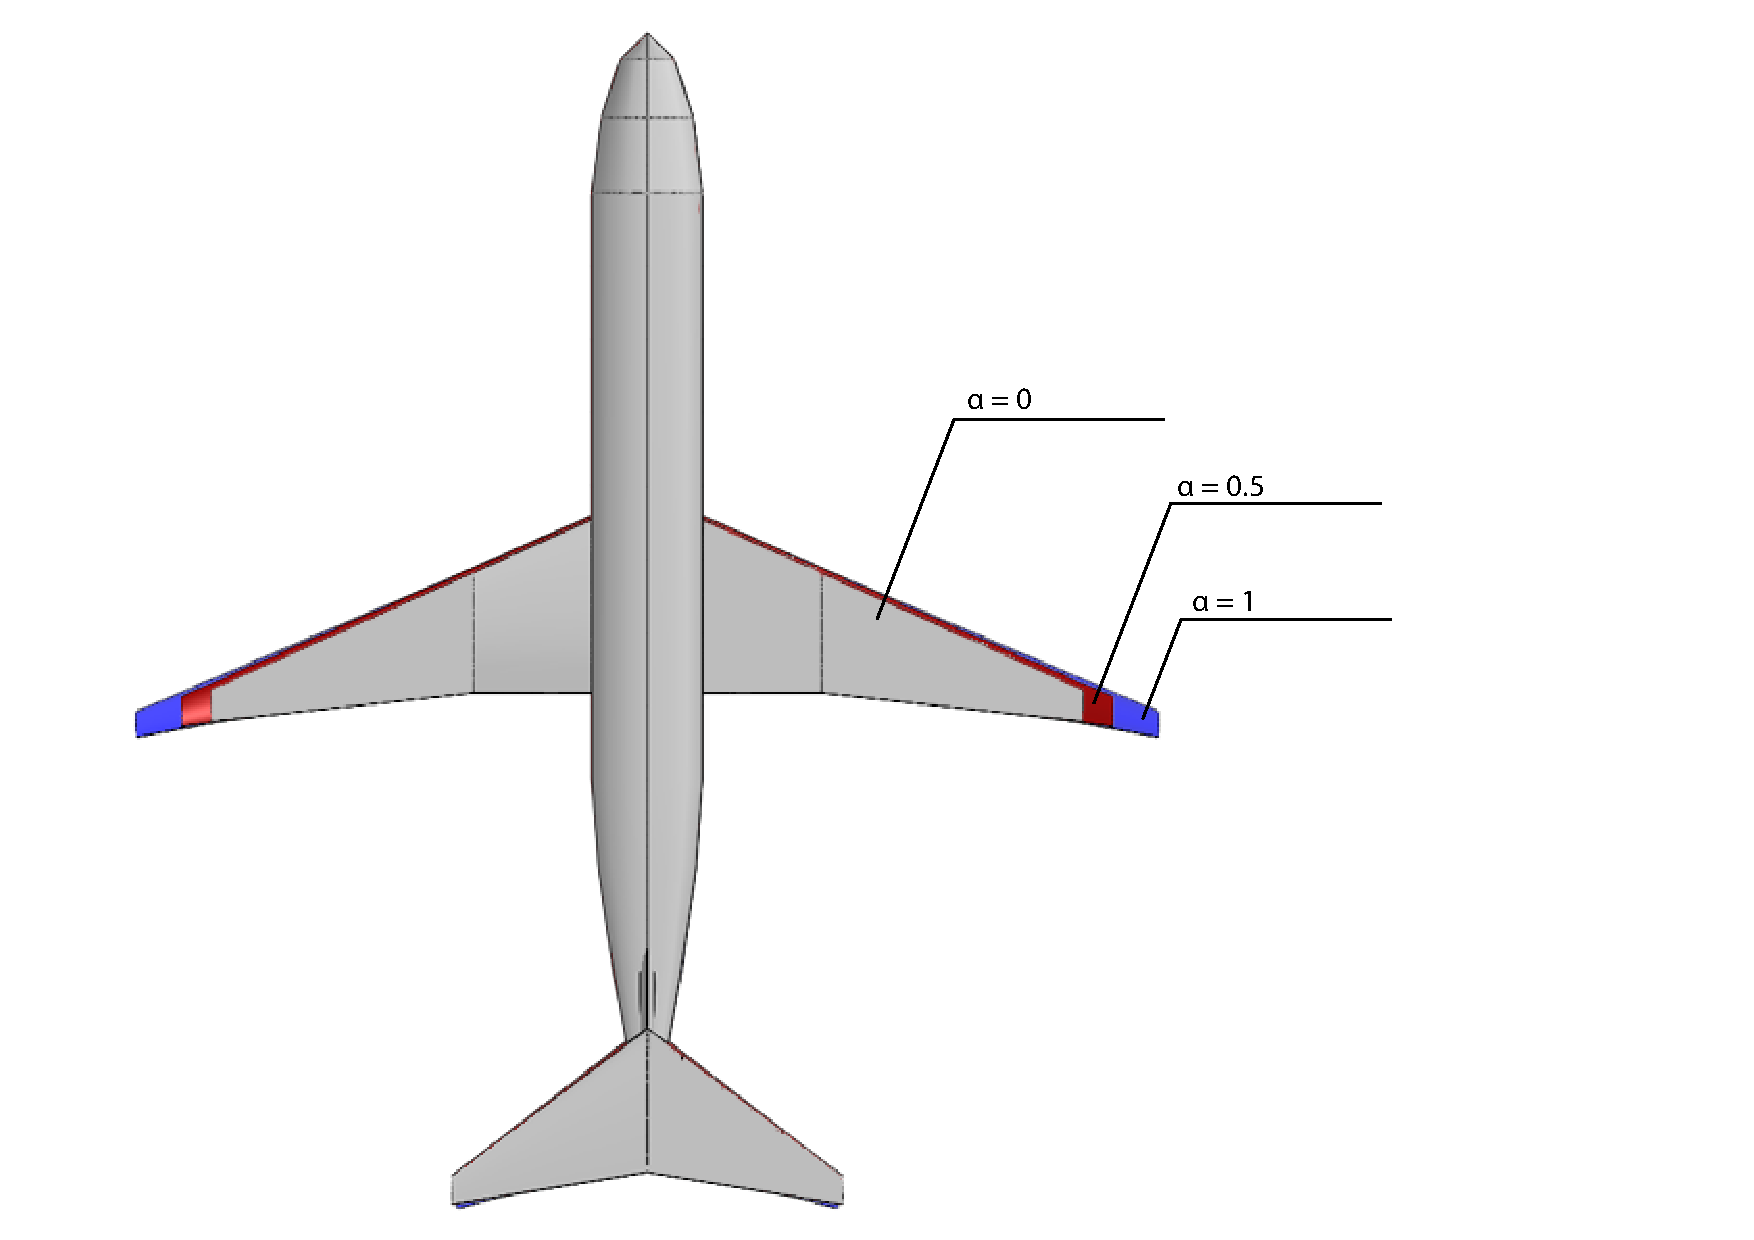
\includegraphics[keepaspectratio, width=0.8\textwidth]{images/chap3/hybrid_dep_pareto_render_comp}
	\caption{Comparison between three different configurations, chosen within the Pareto frontier for $\alpha=0$, $\alpha=0.5$ and $\alpha=1$ in Eq.~\eqref{eq:multiobj_aux_func}.}
	\label{fig:hybrid_dep_pareto_aircraft_render_comparison}
\end{figure}

\section{Conclusion}
\label{sec:chap3_conclusion}

This chapter is deputed to the exploration and performance evaluation of the hybrid aircraft, with distributed electric propulsion, shown in Fig.~\ref{fig:aircraft_dep_concept}. 
Modelisation of the propulsive chain, in all its component, is first described, followed by a revision of sizing procedure, to evaluate performances of the new proposed concept. 
Sensitivity analysis on the electric components' technology is presented, considering pespectives for 2035, to assess their impact on the overall design and define a baseline. 
Then, the hybrid aircraft is studied, for a given set of design ranges, and compared with the A320. 

Results using the MDA show that, for a given set of TLAR and geometrical inputs, the hybrid aircraft is more performing than the baseline up to a certain range, called ``range breakdown'', which is around 1000~nmi.
This behaviour is explained considering that batteries introduce a relevant penalty in weight, which is empty mass carried in cruise: at short ranges, the impact of having a fully electric climb overcomes the effect of a heavier aircraft in cruise, but on longer ranges the batteries' weight diverge soon, making the aircraft so heavy that the baseline shows better fuel and energy consumptions; after 1600~nmi no feasible hybrid aircraft has been achieved. 

Then, the MDO formulation, using the integrated version of FAST and OpenMDAO, is used to optimise the concept. 
Three different configurations, varying the number of engines from 16 to 48, are taken into account, to evaluate the impact of distributed propulsion. 
Trends regarding fuel and energy consumption are similar to the previous case without optimisation, but the ``breakdown range'' is extended up to 1200~nmi because there is more margin of improvement, before reaching the span limit, thanks to the blowing effect over the wing. 
Also, the case with 32 motors is the most performing among the three configurations, because it balances propulsive and aerodynamics efficiency. 
This result descents directly for the MDO peculiarity to consider interaction and coupling between different disciplines, and find the best balance among them. 
A final mission optimisation confirms also that mass penalties introduced by batteries are so relevant, that is more convenient to fly without any electric assisted phase. 

Finally, a Pareto front is obtained, comparing a genetic algorithm and a gradient based algorithm, to assess the advantage of using derivatives in the optimisation process. 
The computational cost in the second case is reduced of more than 70\%, confirming that, despite the great efforts spent in computing analytic derivatives, the computational time is sensitively reduced. 

At this point, the MDO formulation is ready, and it has been demonstrated its capability to deal with the problem of unconventional configuration. 
In particular, it has been shown that it is capable to get all the interactions in an optimisation process, resulting in interesting tradeoff, that with the MDA approach may have been harder to capture. 
Then, the hybrid aircraft configuration is exploited, and thus the left side of the roadmap shown in Fig.~\ref{fig:phd_roadmap} is fully covered. 
In particular, the main conclusion can be drawn is that the hybrid electric concept has a remarked zone of interest for its design, because of the penalties in mass introduced. 
To possibly extend the region of interest, is then of relevance to consider a Blended Wing-Body configuration, which naturally has a high value of LoD. 

Next chapters set up the methodology for the Blended Wing-Body sizing and assess its performance in a similar way than was done in this chapter, in order to explore also the right branch of the PhD roadmap of Fig.~\ref{fig:phd_roadmap}.

\clearpage

\begin{mdframed}[hidealllines=true,backgroundcolor=blue!20]
	\section*{Synthesis of the chapter}
	
	\begin{itemize}
		
		\item The propulsive chain, based on distributed electric propulsion, is modelised and applied to a conventional tube-and-wing, to assess its advantages. 
		
		\item The sizing loop is revised to consider new features of hybrid propulsion. 
		
		\item From a technological point of view, there is a lot of uncertainty in the 2035 perspective: a sensitivity analysis identifies the battery as the most critical component for the sizing. 
		
		\item The proposed tube-and-wing aircraft featuring distributed electric propulsion is explored in terms of performance:
		\begin{itemize}
			
			\item[-] The concept is evaluated against the reference A320 CERAS test case, resized at the same technological level. 
			
			\item[-] The hybrid concept is advantageous up to a specific ``breakdown'' range: due to the presence of batteries, below the range the electrified climb overcomes the penalties in weight; above the range the effect of having empty weight carried in cruise is more relevant. 
			
			\item[-] Fuel consumption may be misleading for the evaluation: energy is more sensitive since it includes the contribution of batteries and power required by subsystems. 
			
			\item[-] Optimisation is carried out considering 16, 32 and 48 engines distributed along the wing: results show that the configuration with 32 engines represents a balance between aerodynamics and propulsion and it is the most performing.
			
			\item[-] Batteries are identified as the main source of penalties in mass: mission optimisation shows that for the fuel reduction is more convenient to remove these elements and generate electric power only by the gasturbines. 
		\end{itemize}
		
		\item For the test case of a Pareto frontier, the computational performance of a gradient-based methods are assessed against a gradient-free method. Results show that the deployment of analytic derivatives reduces the computational cost of about 70\%, which is a key feature for designers. 
		
	\end{itemize}
\end{mdframed}

\clearpage

\begin{mdframed}[hidealllines=true,backgroundcolor=green!20]
	\section*{Research contribution }
	
	\begin{itemize}
		\item[-] \textbf{Conference paper}. A. Sgueglia, P. Schmollgruber, N. Bartoli, O. Atinault, E. Benard and J. Morlier, \emph{Exploration and sizing of a large passenger aircraft with distributed electric ducted fan}, AIAA SciTech 2018 proceedings, Kissimmee, Florida (USA), 2018. DOI: \url{10.2514/6.2018-1745}
		
		\item[-] \textbf{Journal paper}. A. Sgueglia, P. Schmollgruber, E. Benard, N. Bartoli, J. Morlier, J. Jasa, J. R. R. A. Martins, J. T. Hwang and J. S. Gray, \emph{Development of a multidisciplinary design optimization framework with gradient calculation applied to hybrid aircraft}, Journal of Aircraft, 2019. Under review. 
		
		\item[-] \textbf{Book chapter}. A. Sgueglia, S. Dubreuil and N. Bartoli, \emph{Technologies sensitivity analysis of an hybrid aircraft}, Chapter 10 of the book ``Aerospace system analysis and optimization in uncertainty'', edited by L. Brevault, M. Balesdent and J. Morio. Springer Optimization and its Application. New York: Springer, 2019. In press. 
		
	\end{itemize}
\end{mdframed}